% LaTeX Template
% This template is made for project reports
% 	You may adjust it to your own needs/purposesF

% Copyright: http://www.howtotex.com/
% Date: March 2011

%%% Preamble
\PassOptionsToPackage{table}{xcolor}
\documentclass[12pt, a4paper, oneside, slovene]{article}
%\documentclass[paper=a4, fontsize=12pt]{scrartcl}	% Article class of KOMA-script with 11pt font and a4 format

\usepackage[a4paper, left=2.5cm, right=2.5cm, top=2.5cm, bottom=2.5cm]{geometry}
\usepackage[T1]{fontenc}
\usepackage{fourier}

\usepackage[utf8x]{inputenc}
\usepackage[slovene]{babel}															% English language/hyphenation
\usepackage[protrusion=true,expansion=true]{microtype}				% Better typography
\usepackage{amsmath,amsfonts,amsthm}										% Math packages
%\usepackage[pdftex]{graphicx}
\usepackage{graphicx}
% Enable pdflatex

\usepackage{import}
\usepackage{url}
\usepackage{hyperref}

\usepackage{lscape}

%%% Custom sectioning (sectsty package)
\usepackage{sectsty}
% Custom sectioning (see below)
%\allsectionsfont{\normalfont\scshape}	% Change font of al section
                                % commands
\allsectionsfont{\normalfont}	% Change font of al section commands

\usepackage[shortlabels]{enumitem}
\setlist{nosep} %%Zmanjša razdaljo med okolji za seznami in besedilom!cg

\usepackage{setspace}

%%% Custom headers/footers (fancyhdr package)
%%Fancy boxes

\usepackage{fancyhdr}

\setlength{\headheight}{13.6pt}
%\setlength{\footheight}{13.6pt}

\lhead[]{}
\chead[]{}
\rhead[]{}

\lfoot[]{}
\cfoot[\thepage]{\thepage}
\rfoot[]{}


\renewcommand{\headrulewidth}{0pt}			% Remove header underlines
\renewcommand{\footrulewidth}{0pt}				% Remove footer underlines

\usepackage[pdftex,dvipsnames,table,x11names,rgb,html]{xcolor}

\usepackage{wrapfig}

%%%Nastavitve barv
\definecolor{airforceblue}{rgb}{0.36, 0.54, 0.66}

%% \usepackage{solarized-light} to so nastavitve, ki določajo barvno
%% shemo za solarized prenesene so zaradi overleaf.com

%Nastavitve barv za Solarized

\definecolor{sbase03}{HTML}{002B36}
\definecolor{sbase02}{HTML}{073642}
\definecolor{sbase01}{HTML}{586E75}
\definecolor{sbase00}{HTML}{657B83}
\definecolor{sbase0}{HTML}{839496}
\definecolor{sbase1}{HTML}{93A1A1}
\definecolor{sbase2}{HTML}{EEE8D5}
\definecolor{sbase3}{HTML}{FDF6E3}
\definecolor{syellow}{HTML}{B58900}
\definecolor{sorange}{HTML}{CB4B16}
\definecolor{sred}{HTML}{DC322F}
\definecolor{smagenta}{HTML}{D33682}
\definecolor{sviolet}{HTML}{6C71C4}
\definecolor{sblue}{HTML}{268BD2}
\definecolor{scyan}{HTML}{2AA198}
\definecolor{sgreen}{HTML}{859900}

%Nastavitve za prikaz barvanja kode!
\usepackage{listings}
\lstset{
    % How/what to match
    sensitive=true,
    % Border (above and below)
    frame=none,
    % Extra margin on line (align with paragraph)
    xleftmargin=\parindent,
    % Put extra space under caption
    belowcaptionskip=1\baselineskip,
    % Colors
    rulecolor=\color{sbase1},
    backgroundcolor=\color{sbase3},
    basicstyle=\color{sbase00}\ttfamily\footnotesize,
    keywordstyle=\color{scyan},
    commentstyle=\color{sbase1},
    stringstyle=\color{sblue},
    numberstyle=\color{sbase1},
    identifierstyle=\color{sbase00},
    % Break long lines into multiple lines?
    breaklines=true,
    % Show a character for spaces?
    showstringspaces=false,
    tabsize=2,
    numbers=left,                    % where to put the line-numbers; possible values are (none, left, right)
    numbersep=5pt,                   % how far the line-numbers are from the code
    numberstyle=\footnotesize,        %\color{mygray}, % the style
                                %that
   % inputencoding=utf8,
    extendedchars=true,
    literate=
    {š}{{\v{s}}}1
    {č}{{\v{c}}}1
    {ž}{{\v{z}}}1
}

\usepackage{fancyvrb}

%%Barvne škatle
\usepackage{tcolorbox}
%ustvarjanje lastnoe barvne škatle!
\newtcolorbox[auto counter]{examplebox}[2][]{%
colframe=sbase02!100,
colback=sbase3!100,
coltitle=sbase1!100!black,
colupper=sbase01!100!black,
collower=sbase01!100!black,
fonttitle=\bfseries,
title=Primer ~\thetcbcounter: #2,#1
}


%ustvarjanje lastnoe barvne škatle za osebno posameznega portala!
\newtcolorbox[auto counter]{osebnabox}[2][]{%
colframe=sbase02!100,
colback=sbase3!100,
coltitle=sbase1!100!black,
colupper=sbase01!100!black,
collower=sbase01!100!black,
fonttitle=\bfseries,
title= #2,#1
}


\usepackage{xargs}  %Uporabei več kot en argument v novem ukazu
%Paket za dodajanje todo oblačkov!
\usepackage[colorinlistoftodos,prependcaption,textsize=tiny]{todonotes}
%\newcommandx{\unsure}[2][1=]{\todo[linecolor=red,backgroundcolor=red!25,bordercolor=red,#1]{#2}}
\newcommandx{\TODO}[2][1=]{\todo[linecolor=blue,backgroundcolor=blue!25,bordercolor=blue,#1]{#2}}
\newcommand{\inlcomment}{\info[inline]{1=}}
%%% Equation and float numbering
%\numberwithin{equation}{section}		% Equationnumbering: section.eq#
%\numberwithin{figure}{section}			% Figurenumbering: section.fig#
%\numberwithin{table}{section}		        % Tablenumbering: section.tab#

%Nastavitve odstavkov
\setlength{\parindent}{0cm}
\setlength{\parskip}{10px}

%Prostor med vrsticami
%\singlespacing
\onehalfspacing

%%Diferent enumeration
%\usepackage{enumerate}

%%Pandoc workaroun \tightlisr
\providecommand{\tightlist}{%
  \setlength{\itemsep}{0pt}\setlength{\parskip}{0pt}}


%\usepackage[table]{xcolor}
%%Ne preverja če napis gre v eno vrstico in ga zato ne premakne na sredino.
\usepackage[singlelinecheck=false]{caption}


%%% Maketitle metadata
\newcommand{\horrule}[1]{\rule{\linewidth}{#1}} 	% Horizontal rule
%%% Begin document

%%%


%Spremenljivke

%Ustanova
\newcommand{\univerza}{UNIVERZA V MARIBORU}
\newcommand{\fakulteta}{FAKULTETA ZA NARAVOSLOVJE IN MATEMATIKO}
\newcommand{\naslovfak}{Koroška cesta 160, 2000 Maribor}
\newcommand{\oddelek}{Oddelek za matematiko in računalništvo}

%Naslov
\newcommand{\naslov}{DIPLOMSKO DELO} \newcommand{\podnaslov}{Spletni
  portali za učenje programiranja: klasifikacija in možnosti uporabe v
  izobraževanj}

% Mentor/profesor
\newcommand{\mentor}{doc. dr. Igor Pesek}

% Študent
\newcommand{\kandidat}{Gregor Nemec}
\newcommand{\program}{Fizika in računalništvo}
\newcommand{\letnik}{4.letnik}
\newcommand{\smer}{Fizika in računalništvo}
\newcommand{\email}{gregorneme@gmail.com}

% Naslov, datum

\newcommand{\datum}{Maribor, 2016}

%Začetek dokumenta

\begin{document}

\thispagestyle{empty}
%%% Document title variables

%%%%%%%%%%%%%%%%%%%%%%%%%%%%%%%%%%%%%%%%%%%%%%%%%%%%%%%%%%%%%% 
% NASLOVNICA
%%%%%%%%%%%%%%%%%%%%%%%%%%%%%%%%%%%%%%%%%%%%%%%%%%%%%%%%%%%%%% 
\pagestyle{empty}
% ---------======== Naslovnica =======----------
\begin{center}
  \large
  \UNIVERZA

  \FAKULTETA

  \oddelek

\end{center}

\vspace{4cm}


\begin{center}
  \vspace{1cm}
  {\Huge \bfseries \naslov}\\
  \vspace{2cm}
  {\Large \kandidat}
\end{center}
\vspace*{\fill}
\vspace*{\fill}

% \begin{flushleft}
%   % \vspace{1cm}
%   \Large \mentor
% \end{flushleft}

\begin{center}


  \vspace{2cm}


  {\large \datum}
\end{center}


% ---------======== Naslovnica =======----------

%%% Local Variables:
%%% mode: latex
%%% TeX-master: "diploma"
%%% End:

\newpage
\tableofcontents
\newpage
%%Seznam kratic, ki se uporablja čez diplomsko delo.

\section*{Pregled uporabljenih simbolov in označb}
\label{sec:pregled_uporabljenih_simbolov_in_označb}

\begin{enumerate}[leftmargin=*]
\item \textbf{IKT} - informacijsko komunikacijska tehnologija;
\item \textbf{SPUP} - spletni portal za učenje programiranja;
\item \textbf{SPZP} - spletna aplikacija za programiranje;
\item \textbf{AVP} - aplikacijski programski vmesnik
  (\emph{ang. application programming interface \textbf{API}});
\end{enumerate}




%%% Local Variables:
%%% mode: latex
%%% TeX-master: "diploma"
%%% End:

\newpage
\pagestyle{fancy}
\setcounter{page}{1}
\section{UVOD}
\label{sec:Uvod}

% Originalna dispozicija: S trendom popularizacije programiranja, so
% se v zadnjem času pojavili spletni portali, kot je Codeacademy, ki
% omogočajo spletno učenje programiranja in kodiranja. V diplomskega
% dela določite kriterije in z njimi ovrednotite posamezne portale.
% Raziščite možne načine uporabe spletnih portalov in podajte ideje
% kako bi jih lahko umestili v pouk računalništva v OŠ in SŠ.

V svetovnem merilu se pojavlja trend po popularizaciji programiranja
ali kodiranja. V zadnjem obdobju so se na spletu pojavili številni
portali, kot je na primer \emph{CodeAcademy}, ki ponujajo učenje
programiranja. %%%?????

%%ToDO:
%%Kdaj točno se srečajo dijaki s programiranjem in kateri
%%srednješolski program bomo pregledali podrobneje?

%\TODO[inline]{Testiranje todojev} %Uporaba za dodajanje opomb v vrstici!
%\TODO{Testiranje novega ukaza!} %Uporaba za testiranje opomb na robu!

V večini se učenci prvič srečajo s pojmi programiranja pri izbirnih
predmetih \emph{Urejanje besedil, Multimedija in Računalniška
  omrežja}. Dijaki se srečajo s programiranjem v 1. letniku pri
predmetu informatike. Posebnost so strokovni programi, katerim je
osnova računalništvo. Zanimali nas bodo novinci in njihove težave pri
začetnih korakih učenju programiranja. Torej vsi učenci in dijaki, ki
se šele srečujejo s programiranjem.

Najprej se je uporaba spletne tehnologija in nastanek spletnih
portalov za namen učenja programiranja pojavila v akademskem okolju na
posameznih univerzah. Zanimal nas bo razlog za nastanek takšnih okolij
na univerzah, zato bomo pregledali literaturo in poskušali ugotoviti,
zakaj in kako se na višje šolskem področju uporabljajo spletne
tehnologije za poučevanje programiranja.

Izluščili bomo predlagane rešitve za uporabo spletnih tehnologij pri
učenje programiranja. Spoznali bomo kaj so osnovni koncepti
programiranja s katerimi se srečajo novinci in katere so strategije in
metode, ki se pri učenju uporabljajo.

Na podlagi pregledanega bomo določili kriterije in kategorizirali ter
ovrednotili spletne portale. Najbolj bojo zanimivi tisti
spletni portali, ki ponujajo številne programske jezike, urejevalnik
besedil, zaganjanje napisane programske kode in neko obliko odziva, ki
uporabniku omogoča odkrivanje napak.

%%Kateri so programski jeziki primerni za učenje programiranja in
%%kateri so za to določeni v RS.

Ogledali si bomo kje se uči programiranja na osnovni (\textbf{OŠ})in
srednji šoli (\textbf{SŠ}). Pri katerih izbirnih vsebinah, predmetih
in kakšna je vsebina, ki jo predvideva učni nart. Uporabo spletnih
portalov bomo skušali umestiti v pouk OŠ in SŠ tako, da bo njihova
uporaba najbolj koristna in smiselna.


%%% Local Variables:
%%% mode: latex
%%% TeX-master: "diploma"
%%% End:

\newpage
%% UVOD je posebej datoteka zaradi lažjega upravljanja.

\section{Uporaba računalnika v izobraževanju}
\label{sec:uporaba-raunalnika-v}

Model uporabe računalnika v izobraževanju je Gerlič \cite{gerlic_2000}
razdelil na tri področja. V \textbf{primarno področje} lahko uvrstimo
učenje računalništva in programiranja, saj sem prištevamo aktivnosti s
katerimi želimo uporabnike seznaniti z delovanjem in uporabo
računalnika oz. sodobno informacijsko komunikacijsko tehnologijo
(\textbf{IKT}). Računalnik je tista učna vsebina, ki jo obravnavamo
\cite{model_uporabe_rac_izo-web}. \textbf{Sekundarno področje}
predstavlja vse tiste aktivnosti, katere so vezane neposredno na
izobraževalni proces katerega koli predmetnega področja. Računalnik in
IKT nastopata kot učno sredstvo ali pripomoček v oblikah
tradicionalnih računalniško podprtih učnih sistemov ali inteligentnih
ekspertnih sistemov. V \textbf{terciarno področje}, spadajo vse
aktivnosti, ki spremljajo izobraževanje. Sem se štejejo aktivnosti
izobraževanja, vodenja in upravljanja izobraževalnega sistema.

V tem diplomskem delu nas bo zanimalo le \textbf{primarno področje}
uporabe računalnika v izobraževanju, ki je razdeljeno v dveh pomembnih
področjih \cite{gerlic_2000}:

\begin{itemize}
\tightlist
\item kot element \textbf{splošne izobrazbe},
\item kot element \textbf{ožje strokovne} - poklicne izobrazbe
  oz. usposabljanja.
\end{itemize}

\subsection{Splošnoizobraževalno področje}
\label{sec:spološnoiz_področje}

V današnjem času se računalnik kot element splošne izobrazbe kaže kot
velika potreba oz. se zdi znanje njegove uporabe samoumevno. Že pri
najmlajših otrocih računalnik vzbuja zanimanje in interes.  Računalnik
je postal intelektualno orodje in pripomoček v vsaki sferi človekove
dejavnosti in je prodrl tudi v šolo. Tako imenovana \textbf{računalniška
  pismenost} postaja nuja in zajema vse to kar bi človek moral znati o
računalniku in to, kako je potrebno z njim delati, da bo uspešno živel
v družbi, ki je osnovana na informacijah oz. informacijski družbi
\cite{klemencic_2011}.

V zvezi z definicijo in pojmovanjem \textbf{računalniške pismenosti}
se kažeta dve usmeritvi, Gerlič \cite{gerlic_2000} navaja številne
avtorje obeh usmeritev in povzema:

Prva poudarja \textbf{sposobnost računalniškega programiranja} in
opredeljuje s pojmom pismenosti sposobnost branja in pisanja
podobno kot je to značilno za jezikovno pismenost. Tako zagovorniki,
te smeri poudarjajo, da je cilj računalniške pismenosti, učenje in
veščina programiranja z novim načinom mišljenja in strategijami
ugotavljanja in popravljanja računalniških programov.

Druga smer poudarja \textbf{splošno usposobljenost} za delo z
računalnikom in da ni smiselno, da vsak kdo postane programer, zaradi
tega, ker se bo računalnik uporabljal v najširšem smislu v
praksi. Pomembno za učenca je da razume, delovanje računalnika in se
zaveda njegovega vpliva na razvoj družbe. Učencu moramo pomagati, da
dejanske probleme identificira in jih lahko reši že z narejeno
komercialno programsko opremo.

V zgodnjih letih sta bili značilni obe usmeritvi. Pozneje je prišlo do
preobrata leta 1987 po mednarodnem simpoziju na Univerzi v
Stanfordu. Eden od sklepov simpozija je bil ta, da se v
splošnoizobraževalne programe, ne uči več programiranja, še posebej ne
strukturiranih verzij programskega je na primer \textbf{BASIC}, temveč
naj se uči uslužnostne programske opreme, kot je urejevalnik besedil,
orodja za delo z podatkovnimi bazam, grafična grafična orodja itd..


%% Kje je programiranje, ali spada v strokovno izobraževanje in ne
%% spada v splošno računalniško pismenost, ali je danes zahteva po
%% zanju programiranju le to že uvrstila med splošno pismenost.

Ta dejstva je Gerlič \cite{gerlic_2000} povzel leta 2000 in je
predlagal isto usmeritev na: \emph{``Učencem vseh stopenj želimo ob
  čim večjem številu ur praktičnega dela z računalnikom, ob določenem
  problemu in ob uporabi ustreznih komercialnih programov seznaniti z
  osnovami računalništva in informatike.''} V nadaljevanju bomo lahko
ugotovili kakšni so današnji učni načrti za \textbf{OŠ} in \textbf{SŠ}
in ali so se zgornje ugotovitve uresničile in ohranile.

%%Moje misli.
Zanimivo bi bilo preiskati tudi kakšni so ti trendi danes? Ali zaradi
boljše računalniške pismenosti, predvsem mlajših generacij obstaja
potreba in trend, da se programiranje ponudi v širšem kontekstu tudi
na splošnem izobraževalnem nivoju.  Zanima nas koliko je računalniške
znanosti in programiranja v splošnoizobraževalnem področju, saj želimo
pokazati, da spletni portali za učenje programiranja zaradi
tehnološkega napredka omogočajo lažjo pot k učenju programiranja. Zato
nas po pozneje zanimalo kje je umeščeno v učnem načrtu programiranje v
\textbf{OŠ} in \textbf{SŠ}.

%% Podrobneje kje se izvaja računalniško izobraževanje v OŠ in SŠ
%% imamo v posebej zato namenjenem poglavju Računalništvo se ne izvaja
%% kot redni predmet, temveč poteka v

\subsection{Strokovno izobraževalno področje}
\label{sec:strokovno_izo_področje}

%% Gerlič 2000 -> ima večji del tega poglavja namenjenega znanje
%% računalništva za pedagoške delavce.

Sem prištevamo vse tiste aktivnosti, s katerimi želimo udeležence
izobraževanja usposobiti na različnih ravneh tako, da se bodo ti z
računalnikom in informacijskimi sistemi ukvarjali na poklicni ravni
\cite{gerlic_2000}.

%%Tu sem napisal po svoje.
Gerlič raziskuje podrobno strokovno področje na katerem se
izobražujejo bodoči učitelji računalništva. Lahko povemo, da sem
spadajo vse ozko usmerjene računalniške in informacijske smeri srednjih
šol, visokih, višjih ter univerzitetnih študijev. Zanima nas področje
programiranja, kar je predvsem predmet strokovnega
izobraževanja. Čeprav se bomo v diplomskem delu posvetili spletnim
portalom za učenje programiranja na splošnem nivoju, bomo pozneje vso
znanje zlahka prenesli tudi na ožje strokovno izobraževanj, saj je tu
uvod, začetkov programiranja, podoben na vseh težavnih stopnjah.

\subsection{Programiranje v OŠ}
\label{sec:Programiranje_v_OŠ}

Pouk računalništva v OŠ poteka kot izbirni predmet ali kot neobvezni
izbirni predmet. Za začetek bomo navedli kako je definirano
Računalništvo v učnem načrtu za izbirne predmete v osnovni šoli
\cite{ucni_nacrt-izbirni-os}:
\emph{``Računalništvo je
  naravoslovno-tehnični izbirni predmet, pri katerem se spoznavanje in
  razumevanje osnovnih zakonitosti računalništva prepleta z metodami
  neposrednega dela z računalniki, kar odpira učencem in učenkam
  možnost, da pridobijo tista temeljna znanja računalniške pismenosti,
  ki so potrebna pri nadaljnjem izobraževanju in vsakdanjem življenju.
  ''}.

\subsubsection{Izbirni predmet računalništva}
\label{sec:izbirni_predmet_rac}

Izbirni predmeti računalništva so sestavljenih z treh predmetov in jih
učenke in učenci lahko izberejo v tretjem trilerju, v 7., 8. in/ali
9. razredu. Prvi od teh predmetov je \textbf{računalništvo - urejanje
  besedil}, kjer si učenci pridobijo osnovna znanja, ki so potrebna za
razumevanje in temeljno uporabo računalnika. Naslednja dva predmeta
sta \textbf{računalniška omrežja} in \textbf{multimedija}, kjer se ta
znanja spiralno nadgradijo.

%Koliko ur je posamezen izbirni predmet

Zanima nas kje se pri teh predmetih računalništva pojavlja
programiranje. Vsak izmed teh predmetov ima operativne učne cilje tako
razdeljeno, da programiranje najdemo v tretji enoti, ki spada med
dodatne vsebine. Posamezne operativne cilje, dejavnosti in vsebino
prikazuje tabela \ref{tab:cilji_izb_prog}.

\begin{table}[!htb]
  \caption{Operativni cilji, dejavnosti in vsebine izbirnega predmeta
    računalništvo za III. dodatno enoto. \cite{ucni_nacrt-izbirni-os}}.
\label{tab:cilji_izb_prog}
\begin{tabular}{
  | p{0.33\linewidth-2\tabcolsep} |
  p{0.33\linewidth-2\tabcolsep} |
  p{0.33\linewidth-2\tabcolsep} | }
  \hline
  \rowcolor{gray!50}
  \textbf{OPERATIVNI CILJI} & \textbf{DEJAVNOSTI} & \textbf{VSEBINE} \\
  \hline

  \begin{itemize}[leftmargin=*]
    \tightlist
  \item napisati algoritem z odločitvijo, ki reši preprost vsakdanji
    problem;
  \item izdelati in spremeniti računalniški program z odločitvijo.
  \end{itemize}
  &
  \begin{itemize}[leftmargin=*]
  \item analizirati preprost problem;
  \item uporabljati osnovne korake programiranja.
  \end{itemize}
 &
  \begin{itemize}[leftmargin=*]
  \item risanje diagrama poteka za problem z odločitvijo;
  \item izdelava računalniškega programa.
  \end{itemize}
 \\
 \hline

\end{tabular}
\end{table}

Programiranje se pojavlja le kot dodatna vsebine, kar se kaže v
uresničitvi smeri računalništva, ki zagovarja \textbf{splošno
  usposobljenost}, kot smo jo opredelili v poglavju
\ref{sec:spološnoiz_področje}. Vendar se tu učiteljem računalništva
ponuja izjemna priložnost, da z učenci in učenkami naredijo korak v
osnove računalništva in programiranja.

\subsubsection{Neobvezno izbirni predmet računalništva}
\label{sec:neobvezno_izbirni_predmet_rac}

Opredelitev predmeta v učnem načrtu
\cite{ucni_nacrt-neobvezni-izbirni-os}, pravi, da neobvezni izbirni
predmet računalništva učence seznanja z različnimi področji
računalništva, računalniškimi koncepti ter procesi in jih ne učijo
dela z posameznimi programi. Učenci se seznanjajo tehniko in metodami
reševanja problemov, razvijajo algoritmičen način
razmišljanja. Opredelitev zadostuje prvi smeri računalniške
pismenosti, ki zagovarja \textbf{sposobnost računalniškega
  programiranja.}. Ker se v tej diplomski nalogi še posebej posvečamo
programiranju nam učni načrt tega predmeta dosti bolj ustreza in si ga
bomo podrobneje pogledali, saj nam bo pregled operativnih ciljev
služil kot vodilo pri nadaljnjem delu.  Najprej preglejmo splošne
cilje, katere povzemamo po učenem načrtu
\cite{ucni_nacrt-neobvezni-izbirni-os} in jih morajo doseči učenci:
\begin{itemize}
\tightlist
\item spoznavajo temeljne koncepte računalništva,
\item razvijajo algoritmični način razmišljanja in spoznavajo
  strategije reševanja problemov,
\item razvijajo sposobnost in odgovornost za sodelovanje v skupini ter
  si krepijo pozitivno samopodobo,
\item pridobivajo sposobnost izbiranja najustreznejše poti za rešitev
  problema,
\item  spoznavajo omejitve človeških sposobnosti in umetne
  inteligence,
\item se zavedajo omejitev računalniških tehnologij,
\item pridobivajo zmožnost razdelitve problema na manjše probleme,
\item se seznanjajo z abstrakcijo oz. poenostavljanjem,
\item spoznavajo in razvijajo zmožnost modeliranja, strokovno
  terminologijo.
\item  razvijajo ustvarjalnost, natančnost in logično razmišljanje,
\item razvijajo in bogatijo svoj jezikovni zaklad ter skrbijo za
  pravilno slovensko izražanje in strokovno terminologijo.
\end{itemize}

Neobvezni izbirni predmet je namenjen učencem 4., 5. in 6. razreda. V
učnem načrtu so operativni cilji predstavljeni tako, da so temeljni
označeni \textbf{krepko} in izbirni \emph{poševno}. Navedli bomo
tiste, ki so navezujejo na programiranje in strategije reševanja
problemov. Operativni cilji so razdeljeni na vsebinske sklope.

\textbf{Vsebina/sklop: Algoritmi}
\begin{itemize}
\tightlist
\item \textbf{razumejo pojem algoritem},
\item \textbf{znajo vsakdanji problem opisati kot zaporedje korakov},
\item \textbf{znajo z algoritmom predstaviti preprosto opravilo},
\item \textbf{algoritem predstavijo simbolno (z diagramom poteka) ali s
  pomočjo navodil v preprostem jeziku},
\item \textbf{sledijo algoritmu, ki ga pripravi nekdo drug},
\item \textbf{znajo v algoritem vključiti vejitev (če) in ponavljanje (zanke)},
\item \emph{znajo algoritem razgraditi na gradnike (podprograme)},
\item \textbf{znajo povezati več algoritmov v celoto, ki reši neki problem},
\item \emph{razumejo vlogo testiranja algoritma in vedo, da je testiranje
  orodje za iskanje napak in ne za potrjevanje pravilnosti},
\item \emph{primerjajo več algoritmov za rešitev problema in znajo poiskati
  najustreznejšega glede na dana merila},
\item \emph{znajo uporabiti nekatere ključne algoritme za sortiranje in
  iskanje},
\item \emph{poznajo osnovne algoritme za iskanje podatkov}.
\end{itemize}

\textbf{Vsebina/sklop: Programi}
\begin{itemize}
\tightlist
\item \textbf{znajo slediti izvajanju tujega programa},
\item \textbf{znajo algoritem zapisati s programom},
\item \textbf{znajo v program vključiti konstante in spremenljivke},
\item \textbf{ razumejo različne podatkovne tipe in jih znajo uporabiti v
  programu},
\item \textbf{znajo spremenljivkam spremeniti vrednost s prireditvenim
  stavkom},
\item \textbf{znajo v programu prebrati vhodne podatke in jih vključiti v
  program},
\item \textbf{znajo izpisovati vrednosti spremenljivk med izvajanjem programa
  in izpisati končni rezultat},
\item \textbf{v program vključijo logične operatorje},
\item \textbf{znajo uporabiti pogojni stavek in izvesti vejitev},
\item \textbf{razumejo pojem zanke in ga znajo uporabiti za rešitev problema},
\item \emph{razumejo kompleksnejše tipe podatkov (nizi, seznami/tabele) in
  jih znajo uporabiti v programu},
\item \textbf{prepoznajo in znajo odpraviti napake v svojem programu},
\item \emph{znajo popraviti napako v tujem programu},
\item \emph{znajo spremeniti program, da dosežejo nov način delovanja
  programa},
\item \emph{znajo rezultate naloge zapisati v datoteko},
\item \textbf{se seznanijo z dogodkovnim programiranjem},
\item \textbf{so zmožni grafične predstavitve scene (velikost objektov, ozadje, pozicioniranje)},
\item \textbf{so zmožni sinhronizacije dialogov/zvokov},
\item \textbf{so zmožni razumeti in realizirati interakcije med liki in objekt}i,
\item \textbf{ so zmožni ustvarjanja animacij}.
\end{itemize}

\textbf{Vsebina/sklop: Podatki}
\begin{itemize}
\tightlist
\item \textbf{razlikujejo podatek in informacijo},
\item \textbf{razumejo dvojiški sistem zapisovanja različnih podatkov},
\item \textbf{razumejo kodiranje podatkov},
\item \textbf{razumejo, da obstajajo podatki v različnih pojavnih oblikah
  (besedilo, zvok, slike, video)},
\item \emph{poznajo načine predstavitev določenih podatkov in odnose med
  njimi (dvojiška drevesa in grafi)},
\item \emph{vedo za stiskanje podatkov in vedo, da je stiskanje lahko brez
  izgub ali z izgubami},
\item \textbf{pojasnijo razliko med konstantami in spremenljivkami v programu},
%\item \textbf{znajo strukturirane podatke zapisati v tabele z vrsticami in
  %stolpci},
%\item \textbf{opišejo potrebo po urejanju podatkov},
\item \emph{poznajo osnovne algoritme za iskanje podatkov},
%\item \textbf{se zavedajo pomembnosti varovanja osebnih podatkov}.
\end{itemize}

\textbf{Vsebina/sklop: Reševanje problemov}
\begin{itemize}
\tightlist
\item \emph{znajo uporabiti različne strategije za reševanje problema},
\item \textbf{znajo našteti faze procesa reševanja problema},
\item \emph{znajo postavljati vprašanja in ugotoviti, kateri podatki so
  znani},
\item \emph{znajo za podano nalogo izluščiti bistvo problema},
\item \textbf{znajo najti ustrezno orodje, s katerim rešijo problem},
\item \textbf{znajo problem razdeliti na več manjših problemov},
\item \textbf{znajo načrtovati in realizirati rešitev},
\item \emph{za podano rešitev znajo oceniti posledice in vpliv na ``okolje''},
\item \emph{znajo uporabiti znano strategijo v novih okoliščinah},
\item \emph{znajo ustvariti nov algoritem za bolj kompleksne probleme},
\item \textbf{znajo učinkovito sodelovati v skupini in rešiti problem
    z uporabo informacijsko-komunikacijske tehnologije znajo ceniti
    neuspešne poskuse reševanja problema kot del poti do rešitve},
\item \emph{znajo kritično ovrednotiti rešitev in ugotoviti ali rešitev
  uspešno reši dani problem},
\item \emph{znajo kritično ovrednotiti strategijo reševanja problema},
\item \emph{zavedajo se omejitev informacijsko-komunikacijske tehnologije
  pri reševanju problemov}.
\end{itemize}

\textbf{Vsebina/sklop: Komunikacija in storitve}
\begin{itemize}
\tightlist
%\item \textbf{poznajo temeljne ideje o delovanju računalniških omrežij},
%\item \textbf{poznajo glavne storitve računalniških omrežij (e-pošta, splet
  %idr.)},
\item \textbf{znajo uporabiti ustrezna orodja in metode za iskanje po spletu},
\item \textbf{znajo uporabiti različne iskalne strategije v iskalnikih},
\item \textbf{poznajo omejitve pri rabi na spletu najdenih informacij
  (zavedajo se pojma intelektualna lastnina)},
%\item \textbf{znajo prikazati podatke na ustrezen način},
%\item \textbf{poznajo glavna varnostna priporočila v omrežjih in omrežni
  %bonton (netetika)}.
\end{itemize}

Kot smo že povedali smo nekatere cilje izvzeli, čeprav je znanje
računalniških omrežij pomembno, ga z vidika programiranja lahko
izpustimo. Lahko povemo, da nam je večina operativnih ciljev ostala,
saj smo jih lahko izključili le malo. Pridemo do spoznanja, da se v
računalniški znanosti pretežen del znanja vrti okoli programiranja in
reševanja problemov. Z samih ciljev lahko spoznamo tudi samo
zahtevnost snovi. Lahko si upamo napovedati, da jih bomo s pravimi
orodji kot so spletni portali za učenje programiranj tudi lažje
dosegli.

\subsection{Programiranje v SŠ}
\label{sec:Programiranje_v_SŠ}

% Dobor bi bilo, da za programiranje SŠ povzamemo splošni program
% gimnazije. OŠ ima zelo zahtevne cilje, lahko bi jih povzeli in
% dodali noto težavnosti.

%Določiti moramo, kateri srednješolski program bomo povzeli.
%Predlagam, splošno gimnazijo z 4. letnim programom rac in informatika

Pregledali bomo predmet \textbf{informatike}, splošnega Gimnazijskega
programa in \textbf{Računalništvo} Tehniške Gimnazije.

\subsubsection{Informatika - Splošni gimnazijski program}
\label{sec:informatika_splošni_gim_program}

%Koliko je ur informatike?
Predmet \textbf{informatike} se poučuje v prvem letniku splošne,
klasične in strokovne Gimnazije. če povzamemo opredelitev z učnega
načrta \cite{ucni_nacrt-informatika-gim}, ta pravi
naslednje. \emph{``Informatika je splošnoizobraževalni predmet, pri
  katerem se teorija poznavanja in razumevanja osnovnih zakonitosti
  informatike prepleta z metodami neposrednega iskanja, zbiranja,
  hranjenja, vrednotenja, obdelave in uporabe podatkov z digitalno
  tehnologijo z namenom oblikovanja rele- vantnih informacij za
  dograjevanje lastnega znanja in za njegovo predstavitev oziroma
  posredovanje drugim.''}

Poučevanje Informatike obsega \emph{70ur} v 1.letniku, izbirni predmet
obsega \emph{210ur} in maturitetni predmet ima \emph{70 + 210ur}, pri
čemer je \emph{70ur} namenjenih projektnemu delu.

Cilji vsebine predmeta so razporejeni na dve ravni:

\begin{itemize}
\item \textbf{splošna znanja}, v katerih dijaki razvijajo temeljnje
  digitalne kompetence, ki so potrebne za učinkovito uporabo digitalne
  tehnologije pri razvijanju lastnega znanja in za njegovo
  predstavitev oziroma posredovanje drugim;
\item \textbf{posebna znanja}, s katerimi dijaki znanje, veščine,
  osebnostne in vedenjske značilnosti,prepričanja, motive in druge
  zmožnosti splošnega znanja spiralno nadgradijo.
\end{itemize}

Za nas pomembne enote najdemo na drugi ravni, \textbf{posebnih znanj}
v tematskem sklopu \textbf{obdelava podatkov}. Zbrali bomo cilje,
kateri izpostavljajo programiranje. Dijaki:

\begin{itemize}
\tightlist
\item \textbf{Računalniška obdelava podatkov}
  \begin{itemize}
    \tightlist
  \item poznajo vlogo računalniškega programa in razložijo pomen programiranja;
  \end{itemize}
\item \textbf{Algoritmi}
  \begin{itemize}
    \tightlist
  \item  opredelijo algoritem in poznajo temeljne zahteve za algoritem,
  \item poznajo temeljne gradnike algoritma, razvijejo algoritem za
    problem z vejiščem in zanko (do 15 gradnikov),
  \item uporabijo diagram poteka in uporabljeno rešitev utemeljijo,
  \item analizirajo algoritem, ki reši zahtevnejši problem, in ga
    ovrednotijo;
  \end{itemize}
\item \textbf{Programski jezik}
  \begin{itemize}
    \tightlist
  \item opredelijo programski jezik in razložijo njegovo funkcijo,
  \item poznajo temeljne gradnike izbranega programskega jezika,
  \item razložijo njihovo funkcijo in razlago ponazorijo s primeri,
  \item opredelijo strukturirano, objektno in dogodkovno
    programiranje,
    \item ločijo med prevajalnikom in tolmačem in razliko razložijo;
  \end{itemize}
\item \textbf{Programiranje}
  \begin{itemize}
    \tightlist
  \item za dani algoritem izdelajo računalniški program,
  \item opredelijo dokumentiranje programa in razložijo njegov pomen,
  \item analizirajo program in ovrednotijo rezultate, dobljene s
     programsko rešitvijo;
  \end{itemize}
\end{itemize}


%Ali naj še dodam tehniško gimnazijo.
\subsubsection{Računalništvo - Tehniška gimnazija}

Cilje učenja programiranja pri tem maturitetnem predmetu najdemo pod
poglavjem \textbf{Programski jeziki in programiranje}. Cilji so
naslednji, dijaki \cite{ucni_nacrt-teh-gim}:

\begin{itemize}
\item poznajo pomen načrtovanja in sistematične gradnje programa,
\item poznajo pojem algoritma in opredelijo njegove lastnosti
  (razumljivost, končnost, enoumnost, razčlenjenost),
\item opišejo načine zapisa algoritma in jih prikažejo na primeru,
  izdelajo algoritem za lažji problem,
\item opredelijo pojem programskega jezika in razložijo njegovo
  funkcijo,
\item poznajo različne vrste programskih jezikov in jih
  razvrstijo po namenu in uporabi,
\item poznajo temeljne gradnike postopkovnega programskega jezika, razložijo njihove funkcije in
razlago ponazorijo s primeri (zaporedje, vejitev, iteracija),
\item opredelijo strukturirano in objektno programiranje,
\item ločijo med prevajanjem in tolmačenjem in razliko razložijo,
\item poznajo osnovno razvojno okolje,
\item poznajo pojme deklaracija, inicializacija, postopek, konstanta,
  spremenljivka, rezervirana beseda, operator, prioriteta,...
\item ločijo med pojmi izvorna koda, izvršljiva koda in vmesna (byte)
  koda,
\item pridobljeno znanje o tipih in algoritmih prenesejo v programski
  jezik in samostojno rešujejo probleme s pomočjo višjega programskega
  jezika Java,
\item poznajo in uporabijo osnovne in sestavljene tipe podatkov,
\item uporabijo pogojna stavka (if, switch),
\item iteracijo realizirajo z zankami (do, for, while),
\item uporabijo tokove podatkov,
\item pripravijo testne podatke, testirajo delovanje programa in beležijo rezultate testiranj,
\item uporabijo razhroščevalnik,
\item napišejo sled programa,
\item izdelajo dokumentacijo programa,
\item uporabijo metode za delo z objekti razredov Math, String, StringBuffer, Integer, Double ...
\item napišejo definicijo razreda(lastnosti, metode ...),
\item deklarirajo in uporabijo objekte,
\item poznajo vlogo in način izvajanja konstruktorja,
\item uporabijo enkapsulacijo, dedovanje in polimorfizem,
\item poznajo načine za prestrezanje in obravnavo izjem,
\item napišejo programe za enostavne probleme iz okolja,
\item analizirajo program in ovrednotijo rezultate, dobljene s programsko rešitvijo (različni
\item algoritmi urejanja podatkov, različni načini zapisovanja podatkov v datoteke ...),
\item predstavijo delovanje programa,
\item analizirajo in kritično vrednotijo rešitve,
\item \emph{poznajo zahtevnejše tehnike programiranja,}
\item \emph{napišejo program z uporabo zahtevnejših tehnik programiranja.}
\end{itemize}

Cilji določajo zelo podrobno obravnavo snovi programskih jezikov in
programiranja, ki na prvi pogled presega uporabo spletnih portalov za
učenja programiranja.

%Ali so spletni portali koristni pri uporabi z strokovnimi predmeti.

\section{Računalniška znanost in programiranje}
\label{sec:računalniška_znanost_in_programiranje}

Računalniška znanost ima številne različice definicij, v grobem jo
lahko definicijo strnemo v naslednjih trditvah \cite{guideTCS}.

\begin{itemize}
\tightlist
\item Ukvarja z značilnostmi tisktega kar je izračunljivo.
\item Je znanost, ki izhaja iz več področij in ime korenine v matematiki,
znanosti in inženirstvu.
\item Ima mnoga podpodročja in je interdisiplinarna z biologijo,
ekonomijo, medicino, zabavo.
\item Ime računalništvo ali računalniška znanost nas lahko tudi zavede in
jo zamenjamo z področjem uporabe računalnika.
\end{itemize}

%Še je potrebno dodati kakšno definicijo z druge literature.

\subsection{Zgodovina programskih jezikov}
\label{sec:zgodovina_programskih_jezikov}


%Splošna zgodovina uporabe računalništva v izobraževanju
%Razdeljeno imam zgodovino rac. v izobrazevanju in programiranje v
%izo, ali je naj vse skupaj. Na kratko dodaj računalniška obdobja, kot
%jih je predstavil Gerlič


Uporaba računalništva v izobraževanju je bila deležna številnih
sprememb. Sama uporaba računalnika v izobraževanju je tesno povezana z
razvojem računalnikov.  Začetno obdobje, 1960 letih prejšnjega
stoletja so računalniki bili zelo dragi in veliki glavni računalniki (
\emph{ang. mainframe} ), na njih se je učilo programiranja, a so se
uporabljali tudi za druga področja.  V tem obdobju se je za učenje
programiranja uporabljal \textbf{FORTRAN} ali
\textbf{asembler}. Programi so bili majhi in enostavi, zaradi fizičnih
omejiteh takratnega delovnega pomnilnika. Temu začetnemu obdobju pravimo
\textbf{terminalsko obdobje} \cite{gerlic_2000}.

V 1970 so na trg prišli manjši računalniki, ki so bili tudi cenejši in
zmogljivejši. V tem času pride v ospredje strukturirano programiranje.
Najpopularnejši programski jezik je bil \textbf{PASCAL}. Predstavnimi
obdobja \textbf{mikroračunalnikov} so bili \emph{Commodore 64,
  Sinclare ZX-81, Apple II}.

V 1980 so se prvič pojavili \textbf{samostojni osebni računalniki}. Programski
jeziki v tem obdobju so bili strukturirani in močnega tipa (
\emph{ang.  strong type.} ). Med te spada \textbf{Ada, Modul 2, ML in
  naj omenimo še Prolog}.

V naslednjem desetletji, 1990 so v ospredje prišli objektno
orjentirani programski jeziki, kot sta \textbf{C++} in \textbf{JAVA}
\cite{thesisAWebP}.



% //Umestitev računalnik v izobraževanju na primarnem področju.
% -\textgreater{} Gerlič Uporaba računalika v namene učenje računalništva
% in programiranja.

% //Doodaj generacije programskih jezikov. //Dodaj vrste programskih
% jezikov.

Metode poučevanja računalništva so se prav tako spreminjale. 1960 so
računalnike uporabljali samo za poučevanje programiranja. Povdarek pri
predmetih programiranja je bil predvsem na detaljlih zmožnosti
programskega jezika. Programiranje je bilo omejeno le na reševanje
enostavnih primerov in povdarek ni bil na reševanju problemov na
splošno.

V 1970 je reševanje problemov in abstrakcija podatkov postala glavni
in najpomembnejši del vseh programerskih predmetov, kar velja še
danes.  Programi so postali večji, bolj interaktivni in spremenil se
je vnos podatkov z tekstovnega v grafičnega. Vsebina predmetov
računalništva se je hitro razširjala, kakor so se množili številni
programski jeziki \cite{thesisAWebP}.

Posebno mesto v izobraževanju ima programski jezik
\textbf{LOGO}. Z ekipo ga je Seymour Papert. Značilnost programskega
jezika je ta, da z programsko kodo rišemo grafiko, ki jo lahko
predstavimo na zaslonu ali z \emph{``z želvo''}, ki se premika po tleh
z ukazi in riše sliko na podlago. Programski jezik je bil prvič
zasnovan v namene učenja programiranja.

%Dodaj slike logo + želva!

% //Misel: V izobraževanju je potrebno previdno izbrati obseg in področja
% vsebin, pri čemer ne smemo zanemariti timsko delo.

\subsection{Osnovni pojmi}
\label{sec:kaj_je_programiranje}

%% Splošne definicije programiranja.
%% Ni le pisanje kode temveč tudi uspešno reševanje nalog in
%% problemov?

Preden nadaljujemo moramo razjasniti nekaj osnovnih pojmov, ki se
pojavljajo računalniški znanosti.

\subsubsection{Program}
\label{sec:program}

Računalniški program je zbirka navodil, ki opravlja točno določeno
nalogo in jo izvajamo na računalniku. \textbf{Centralno procesna
  enot}a je tista, ki izvajanje programa omogoča. Računalniški program
navadno napiše \textbf{programer} v nekem \textbf{programskem jeziku},
postopku pisanja programa pravimo \textbf{programiranje}. Programski
jezik omogoča, da je program zapisan v takšni obliki, da je berljiv za
ljudi in je zapisan v \textbf{izvorni kodi}. Da računalnik razume
napisan program, ga prevede \textbf{prevajalnik
  (\emph{ang. compiler})} v \textbf{strojno kodo.}
\cite{wiki:computer_program}.

\subsubsection{Algoritem}
\label{sec:algoritem}

Z besedo algoritem ponazarjamo postopek, ki je zgrajen z posameznih
operacije in se izvajajo po posameznh korakih. Algoritem daje rešitev
za izračune, procesiranje podatkov, avtomatizacijo postopkov.
Ime besed \emph{``algoritem''} prihaja z imena \textbf{Al-Khwārizmī},
Perzijskega matematika, astronoma, geografa in učenjaka \cite{wiki:algorithem}.

Pri pregedu učnih načrtov v poglavju
\ref{sec:neobvezno_izbirni_predmet_rac} smo lahko zasledili cilje kot
so:

\begin{itemize}
\tightlist
\item \textbf{znajo vsakdanji problem opisati kot zaporedje korakov},
\item \textbf{znajo z algoritmom predstaviti preprosto opravilo},
\item \textbf{algoritem predstavijo simbolno (z diagramom poteka) ali s
  pomočjo navodil v preprostem jeziku}.
\end{itemize}

% Poglejmo nekaj primerov, kako lahko s pomočjo spletnih portalov za
% učenje programiranja zadostimo tem ciljem in kaktere informacije
% najdemo. Na strani \href{https://code.org}{code.org}. Podroben opis
% strani je v poglavju x.x. Algoritmov se učijo že najmlajši udeleženci
% zato si pri lažjem raumevanju pojma algoritem lahko pomagamo, z
% pristopom \textbf{računalništva brez računalnika}. Spodaj prikazujemo
% dva primera.

Prikazali bomo več različnih predstavitev algoritma, najprej bomo
rešitev zapisali v pesedilni obliki, zatem bomo rešitev podali z
diagramom poteka, na koncu bomo rešitev podali še z programskim
jezikom Scratch in Python.  Za primer bomo prikazali primer algoritma,
ki reši naslednjo nalogo.

%Možnost programskih primerov v takem slogu.

%Dodaj diagram poteka!

\begin{examplebox}[label={prog:al01}]{Algoritem - Najdi največje število}
Algoritem med podanimi števili poišče največje število.

Postopek zapisan v \textbf{besedilu}:
\begin{enumerate}
\tightlist
\item Zapišemo si začetno število, naj bo $0$.
\item Števila v seznamu preglejujemo po vrsti.
\item Vsakič, ko najdemo večje število, ko je naše začasno število,
\item To začasno število prečrtamo in napišemo tisto z seznamoa, ki je
  večje.
\item Postopek ponavljamo, dokler ne pridemo na konec seznama.
\end{enumerate}


% Tu bi bilo dobro, da bi lahko prikazal tekst in sliko v eni vrsti.
Podprogram v \textbf{Scratchu}:

%\begin{figure}
    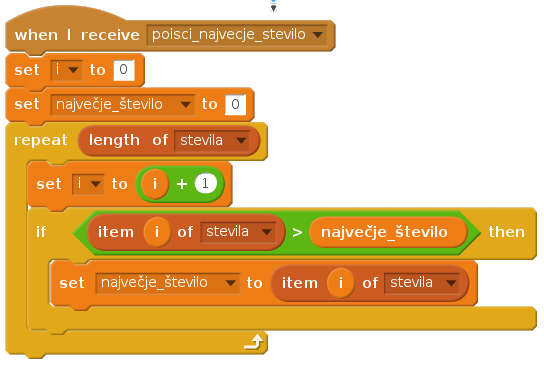
\includegraphics [width=0.6\linewidth, keepaspectratio =
    1] {./images/scratchImg/01-Scr_Alg-NajvecjeSt-img_trs.png}
    % \caption{Test}
    % \label{fig:scr:01-Alg_najdiNajvecje}
%\end {figure}

Podprogram v \textbf{Pythonu}:

\begin{lstlisting}[language=Python]
def najdiNajvecjeStevilo(seznam):
    """Funkcija poisce najvecje stevilo v seznamu."""
    i = 0
    najvecje_stevilo = 0
    for i in range(len(seznam)):
        if seznam[i] > najvecje_stevilo:
            najvecje_stevilo = seznam[i]
    return najvecje_stevilo
\end{lstlisting}
\end{examplebox}



\subsubsection{Programiranje in kodiranje}
\label{sec:programiranje_kodiranje}

Izraz programiranja smo že spoznali. Veliko krat slišimo tudi izraz,
\textbf{``kodiranje'' (\emph{ang. coding})}. Povedali bi lahko da
izraz pomeni, pisanje programske kode, konček izdelek, tisto kar na
koncu damo \textbf{prevajalniku}, kar je \textbf{izvorna koda}, da
prevede v \textbf{strojno kod}o, katero lahko potem zaganjamo.

Za vsakim programiranjem stoji seveda nek programer, lahko bi rekli,
da je za vsakim kodiranjem nekdo, ki mu pravimo
\textbf{koder}. Programer in koder stav veliko krat, dana v isti koš,
vendar si to čisto ne zaslužita, saj je programer, nekdo ki načrtuje
rešitve, na različne načine in z razčličnimi orodji preden sploh
zapiše kaj programske kode. Koder po drugi strani je tista oseba, ki
se dobro spozna na programske jezike vendar, dela veliko krat po
načrtu programera, je tisti ki na kocu zapiše rešitve in je pri tem
zelo unčikovita. Čeprav se ta dva poklica zelo povezana in so meje med
njima tudi veliko krat zabrisane sploh, če je programer in koder ena
in ista oseba \cite{web:coder}.

Pri samem poučevanju računalništva, lahko menimo, da je v prvi vrsti
pomembno to, da se učimo strategije reševanja problemov, torej kako
poučevati, da bo čim več učencev postalo dobrih programerjev.

\subsubsection{Urejevalnik besedil}
\label{sec:urejevalnik_besedil}

Dober urejevalnik besedi lahko programerju lajša delo s številnimi
zmožnostmi. Opisali smo nekatere, saj nam bodo te pomagale lažje
prepoznati dober urejevalnik besedil.

%Podrobneje opiši zmožnosti urejevalnika besedil.

\begin{itemize}
\item Barvanje rezerviranih besed prog. kode.
\item Samodejno zamikanje vrstic programske kode.
\item Ponujanje predlog za samo dokončevanje rezerviranih
    besed in funkcij prog. jezika
\item Izpis opis funkcij z atributi.
\item Samodejno zaključevanje oklepajev.
\end{itemize}

\subsubsection{Integrirano razvojno okolje (\emph{ang. Integrated
    development environment \textbf{IDE}})}

\subsection{Programske paradigme}
\label{sec:programske_paradigme}

Paradigma je način kako obravnavamo in gledamo na stavri, je okvir v
katerem leži naša interpretacija realnosti sveta. Paradigma
najpogosteje pomeni vzorec delovanja v znanstvenem ali drugem
raziskovanju.  Izraz programske paradigme je več pomenka, ki povzema
mentalne procese, strategije reševanja problemov, povezave med
različnimi paradigmami, programske jezike, stil programiranja in še
več (Wikipedia: Paradigma) \cite{guideTCS}.

%//Glavna definicija.
Programske paradigme so hevristike, ki se uporabljajo za reševanje
problemov. Programska paradigma analizira problem, čez specifičen
pogled in na ta način formulira rešitev za dani problem, ki ga razdeli
na manjše dele med katerimi definira razmerja.

Programske paradigme so na primer proceduralno, objektno orientirano,
funkcijsko, logično in istočasno programiranje.

V nadaljevanju bomo spoznali značilnosti programske paradigme
objektnega programiranja, saj je ta v zadnjih letih naj bolj
popularna.

\subsubsection{Objektno orientirano programiranje}
\label{sec:objektno_orijentirano_programiranje}

%V objektno orientiranem \textbf{OO} pristopu programer raz

V objetno orientirano \textbf{OO} programiranje je način kako
programerji razmišljajo o svojem delu. Princip OO model realnosti
sveta predstavlja v \textbf{razredih \emph{ang. class}}. Z takim
načino zapisa programske kode je ramišljanje o programu dosti bolj
naravno \cite{shaums}.

Objekt je predstavnik različnih stvari, ki jih želimo predstavljati v
programskem razredu. Te stvari so lahko kar koli, od realnih objektov
in vse do konceptov. Podajmo primer objekta mačke. Mačka ima številne
karakteristike, kot so barva, ime, teža \dots, tem lasnostim pravimo
da so lasnosti objekta. Mačka je živo bitje, zato njeno početnje, kot
je mjavkanje, spanje, igranje \dots, dejanjem mače pravimo, da so
metode objekta. Pri objetih lahko uporabimo analogijo in objekte
poimenujemo z samostalniki, metode so glagorli in vrednosti lasnosti
objekta so pridevniki. V nadaljevanju si bomo ogledali nekatere
značilnosti, ki definirajo ne programski jezi kot OO \cite{OO-JS}.

\begin{description}
\item[Razred (\emph{ang. Class}):] V resničnem življenju lahko objekte
  združujemo po nekih določenih kriterijih. Orel in sinička sta oba
  ptiča, zato jih lahko damo skupaj v razred katerega poimenujemo
  Ptiči. Razredi so načrti ali recepti za objekte, tako lahko
  ustvarimo več objektov iz istega razreda, saj je razred le shma.
\item [Enkapsulacij (\emph{ang. Encapsulation)}:] je koncept ,ki
  predstavlja, da so podatki, torej \emph{lasnosti} objektov in
  opravila, ki jih lahko opravljajo ali \emph{metode} objektov,
  združeni.
\item [Združevanje (\emph{ang. Aggregation}):] pomeni, da lahko več
  objektov združimo v en objet. To predstavlja močno orodje pri
  razčljenjevanju problemov na manjše pod probleme.
\item [Dedovanje (\emph{ang. Inheritance}):] je eleganten način kako
  porabimo eno kodo več krat. Podajmo primer, imamo splošen razred
  Oseba, ta ima lasnosti kot je ime, datum rojstva in ima napisane
  metode, ki prestavljajo funkcionalnost kot je, da Oseba lahko
  govori, hodi, je, spi. Zatem bi želeli bolj specifičen razred ko je
  Programer. Lahko bi vso kodo ponovno napisali in ji dodali
  specifično za programerja. Dedovanje omogoča, da povemo da Programer
  deduje od razreda Osebe in si tako prihranimo velik del dela.
\item [Polimorfizem (\emph{ang. polymorphisem}):] je način kako lahko
  isto ime metode uporablja več različnih razredov in posledično
  objektov neglede nato, da je najverjetneje koda v njem
  različna.
\end{description}

Programsko paradigmo OO programiranja smo povzeli na kratko, da bi
lažje razumeli zakaj je tako popularna. V nadaljevanju bomo spoznali,
da je večina programskih jezikov, ki se uporabljajo dan danes OO ali
vsaj vsebijejo nekaj lasnosti OO programskih jezikov.

\subsection{Programski jeziki}
\label{sec:programski_jeziki}

V tem poglavju bomo povzeli osnovne značilnosti posameznij programskih
jezikov.  Če na spletu v spletnem iskalniku podamo zahtevo
po najpopularnejšuh programskih jezik, dobimo podobne rezultate
večih spletnih strani\footnote{Pridobljeno 27.04.2016 iz,
  \url{http://www.tiobe.com/tiobe_index}.}  \footnote{Pridobljeno
  27.04.2016 iz, \url{http://githut.info/}.}\footnote{Pridobljeno
  27.04.2016 iz, \url{http://pypl.github.io/PYPL.html}.}  in sicer: \textbf{JAVA,
  C, C++, Python, C\#} v top 10 za nas pomembne majdemo še
\textbf{Java Script}. % in \textbf{Ruby}.

Programski jeziki v izobraževanju so se skozi zgodovino menjavali,
tako kot se je rezvijala računalniška znanost, kar smo že povzeli v
poglavju \ref{sec:zgodovina_programskih_jezikov}. Zanima nas, kateri so
prograsmki jeziki, ki so najbolj primerni za uporabo učenja
programiranja in se uporabljajo danes.

Vsak programski jezik bomo z kratim primerom tudi predstavili z
primerom programske, kode tako bomo dobili lažjo predstavo kakšna je
razlika v sintaksi.

Večina od zgoraj naštetih programskih jezikov je \textbf{OO} razen
izjeme \textbf{C}-ja, ki je predhodnik \textbf{C++}.

%Podajmo še razliko med programsimi jeziki, ki so za večnamesko uporabo
%in tistimi, ki jim pravimo, da imajo ožjo uporabnost.

%Razlika med prevajanimi in tolmačenimi prog. jeziki
%Uredi ker je zmazek

%% Napiši še kaj o generacijah programskih jezikov.

Za nas bodo z izobraževalnega vidika zanimivi predvsme tisti, ki se
uporabljajo pri nas.

\subsubsection{Java}
\label{sec:pj:JAVA}

Java je več namenski programski jezik, njegova osnov so \emph{razredi}
in je OO. Njegova glavna prednost je, da napisano kodo lahko zaganjamo
ne glede na platformo na kateri teče, torej so napisani programi
neodvisni od operacijskega sistema, ki ga poganja računalnik. Zato je
za vsako platformo prilagojen \textbf{virtualni stroj za Javo
  \emph{(ang Java Virtual Machin (JVM)}}, ki prevedeno kodo
poganja. Sintaksa programskega jezika je zelo podobna
\textbf{C++}. Popularnost programskega jezika je še izboljšal zaradi
operacijskega sistem za tablice in telefone \textbf{Android}, ki prav
tako teče na različici (JVM) oz so programi napisani v Javi
\cite{wiki:java}.

V izobraževanju je Java postala zelo priljubljena, prav zaradi
zmožnosti, poganjanja programov na različnih platformah. Uporablja se
na primarnem področju izobraževanja, predvsem na srednjem in visokem
šolskem področju. V sekundarnem področju izobraževanj se je uporabila
predvsem za pisanje programske opreme, ki dopolnjuje izobraževanje,
kot so fizikalne simulacije (\emph{fizleti}) in podobno. Eden od
razlogov, da se je Java na tem področju dobro uveljavila je tudi ta,
da omogoča zagon aplikacije s spletnega brskalnika, vendar je za to
potrebna instalacija posebnega vtičnika, ki to omogoča. Primer
\ref{prog:java01} prikazuje sintakso \emph{"Dobrodošel svet"}
napisanega v Javi.
%Ali moram podati referenco za te Hello world programe.
%http://www.programmingsimplified.com/java-source-codes
\begin{examplebox}[label={prog:java01}]{Program napisan v javi}
\begin{lstlisting}[language=Java]
class First {
   public static void main(String[] arguments) {
     System.out.println("Dobrodosel svet!");
  }
}
\end{lstlisting}
\end{examplebox}


\subsubsection{C++}
\label{sec:pj_c++}

C++ je vse namenski programski jezik, ki je OO in je bil zasnovan kot
sistemski programski jezik. Večina operacijskih sistemov je danes
napisana v kodi C++ in predhodnika C. Kodo programskega mora prevesti
prevajalnik preden jo lahko zaganjamo, za vsako platformo moramo
prevajati posebej.  C++ velja za najhitrejši programski jezik, z njim
lahko opravljamo tako naloge, kot je neposreden nadzor nad
polnilnikom, kot tudi vse višje funkcije, ki jih omogoča. Zato velja
za enega težje učljivih programskih jezikov. Programiranje v C++ se
uči predvsem na višjem in univerzitetnem izobraževalnem nivoju \cite{wiki:cpp}.

%https://en.wikibooks.org/wiki/C%2B%2B_Programming/Examples/Hello_world
\begin{examplebox}[label={prog:cpp01}]{Program napisan v C++}
\begin{lstlisting}[language=C++]
// 'Hello World!' program
#include <iostream>

int main()
{
  std::cout << "Hello World!" << std::endl;
  return 0;
}
\end{lstlisting}
\end{examplebox}

\subsubsection{Java Script}
\label{sec:pj_JS}

\textbf{Java Script (JS)} se je razvil z potrebe po bogatejših in dinamičnih
spletnih straneh. Začetek spleta so predstavljali statični dokumenti,
ki so bile povezane z hiper povezavami. Skirptni jezik z imenom Java
script se je prvič pojavil z spletnim brskalnikom \emph{Netscape
  2.0}. Takrat je bilo možno vstavljanje kratkih odsekov kode, ki so
spletne strani naredile dinamične. Težnja po standardizaciji
skriptnega jezika se je pojavila ko se je na trgu pojavil
\emph{Internet explorer 3.0}, saj je ta imel svojo različico sriptnega
jezika \emph{JScript}. Sedaj se standardni jezik imenuje \textbf{ECMA
  Script} oz. točneje \textbf{ECMA-262}, ki opisuje glavne dele
programskega jezika JavaScript brez specifikacij, spletnega
brskalnika \cite{OO-JS}.

Če smo v prejšnjih poglavjih govorili, da sta bila \textbf{Java} in
\textbf{C++} večnamenska jezika, je JS bil eden tistih, ki so tekli
znotraj vgrajenega gostiteljskega okolja, kot je spletni
brskalnik. Danes imamo tudi okolja, ki omogočajo, da JS teče na
strežnih, na namizju in mobilnih napravah. Torej, kljub zgoraj
omenjeni omejitvi, postaja prav tako večnamenski skriptni programski
jezik. V spodnjem primeru \ref{prog:js01} imamo primer programa
\emph{``Dobrodošel svet!''}, z \textbf{HTML} ogrodjem. Tako programska
kodo odpremo v spletnem brskalniku. Del skriptnega jezika se začne z
značko \texttt{<script type="text/javascript"> JS koda
  </script>}. Povejmo še to, da se koda programskega jezika ne
prevaja, temveč jo poganja \textbf{tolmač}.


%https://en.wikibooks.org/wiki/JavaScript/First_Program
\begin{examplebox}[label={prog:js01}]{Program napisan v JavaScriptu +
    HTML ogrodje}
\begin{lstlisting}[language=Html]
<!DOCTYPE html>
<html lang="en">
  <head>
    <title>Some Page</title>
    <script type="text/javascript">
      alert("Hello World!");
    </script>
  </head>
  <body>
    <p>The content of the web page.</p>
  </body>
</html>
\end{lstlisting}
\end{examplebox}

\subsubsection{Python}
\label{sec:pj_python}

\textbf{Python} je zelo pogosto uporabljen večnamenski programski
jezik. Njegovo kodo podobno kot JS poganja tolmač. Zasnovan je tako,
da je koda čim bolj berljiva in njegova sintaksa omogoča, da
programske koncepte zapišemo v čim manj vrsticah, kakor bi jih lahko v
Javi ali C++. Če so posamezni odseki ali bloki programske kode pri
Javi in C++ označeni z zavitimi oklepaji (``{}''), jih v Pythonu
označimo z tabulatorskim zamikom. V Pythonu lahko uresničimo več
programskih paradigem, kot je OO ali proceduralno
programiranje. Omogočen je dinamičen tip spremenljivk, ima urejeno
avtomatsko upravljanje z pomnilnikom in ima veliko standardno
knjižnico \cite{wiki:python}.

%Kje to piše, da je priporočljiv jezik v SŠ
Pyon se veliko uporablja tudi v izobraževalne namen. Pri nas se
priporoča za začetke učenja programskega jezika na srednjem šolskem
izobraževalnem nivoju. Zaredi tega, ga bomo v diplomskem delu
uporabljali, ko glavni demonstracijski programski jezik.

%https://en.wikibooks.org/wiki/JavaScript/First_Program
\begin{examplebox}[label={prog:py01}]{Program napisan v Pythonu
    HTML ogrodje}
\begin{lstlisting}[language=Python]
print (``Hello world!''')
\end{lstlisting}
\end{examplebox}

\subsection{Osnovni koncepti programiranja}
\label{sec:Osnvni koncepti_programiranja}

% Predstavljeni koncepti na primerih eden OŠ Scratch drugi Python.
V naslednjem odstavku se bomo vprašali kako lahko formuliramo sintakso
programskega jezika? In kaj je npr. definicija \emph{kopice}.V ta
namen definiramo mehko idejo po avtorju Hazzan \cite{guideTCS}, ki je
naslednja. Mehka ideja je koncept, ki mu ne moremo pripisati toge,
niti formalne definicije. Mehke ideje ni niti možno opisati z točno
določeno aplikacijo. Na tem mestu se postavlja vprašanje kako lahko
defineramo nekaj kar se odvija po korakih.

Da odgovorimo na zgornji dve vprašanji, lahko povemo, da so pravila
sintakse togi orisi pri pisanju programske kode in da so semantična
pravila mehke ideje. Opozorimo še na to, da koncepti v računalniški
znanosti niso le toga pravila ali samo mehke ideje, temeč skupek
obojega. V spodnji tabeli \ref{tab:koncept_spremenljivka} prikazuje
primer spremenljivke.

\begin{table}[!h]

\caption{Prikaz dvojnih, togih in mehkih orisov idej na primeru
  spremenljivke \cite{guideTCS}. }
\label{tab:koncept_spremenljivka}
\begin{tabular}{
  | p{0.30\linewidth-2\tabcolsep} |
  p{0.30\linewidth-2\tabcolsep} |
  p{0.40\linewidth-2\tabcolsep} | }
  \hline
  \rowcolor{sbase01!100}
  & \textbf{togi orisi} & \textbf{mehki orisi}\\
  \hline
  ime spremenljivke & Pravilo sintakse. & Potreba po imenu
                                          spremenljivke. Katero ime
                                          spremenljivke je pomembno in
                                          zakaj ga je potrebno
                                          določiti.\\
  \hline
  vrednost spremenljivke & Pravila tipa spremenljivke. Rezervacija
                           pomnilnika. & Spremenljivka ima eno
                                         vrednost, ki se lahko
                                         spreminja s časom.\\
  \hline
  dodelitev začetne vrednosti & Pravila sintakse. & Pomen dodelitve
                                                  začetne vrednosti\\
  \hline

\end{tabular}
\end{table}

V nadaljevanju bomo pregledali in skušali razložiti osnovne koncepte
pri programiranju. Z primerom bomo pokazali enega izmed načinov, kako
jih prestavimo. Za vodilo bomo uporabili učni načrt za OŠ, ki smo ga
pregledali v poglavju \ref{sec:neobvezno_izbirni_predmet_rac} in SŠ,
ki je v poglavju \ref{sec:Programiranje_v_SŠ}. Primeri programov, ki
jih bomo uporabljali in prilagodilo so povzeti s knjige in spletne
strani \emph{``Learning python the hard way''} \cite{web:PTHardWay}.


%%Lahko podamo primere programov z problemskim navodilom in rešitvijo
%%v Pythonu in Scratchu, kjer je to možno.

\subsubsection{Spremenljive}
\label{sec:spremenljivke}

V tem poglavju bomo uresničili naslednje cilje vendar smo jim nekoliko
spremenili vrstni red:
\begin{itemize}
\tightlist
\item \textbf{znajo izpisovati vrednosti spremenljivk med izvajanjem programa
  in izpisati končni rezultat},
\item \textbf{znajo spremenljivkam spremeniti vrednost s prireditvenim
  stavkom},
\item \textbf{znajo v program vključiti konstante in spremenljivke},
\item \textbf{ razumejo različne podatkovne tipe in jih znajo uporabiti v
  programu},
\item \textbf{znajo v programu prebrati vhodne podatke in jih vključiti v
  program},
\end{itemize}

Osnovno interakcijo z računalnikom lahko opišemo na naslednji
način. Računalniku damo neke vhodne podatke, ta podatke po navodilu
programa obdela in nam poda rezultate na neko izhodno naprava. Ta
izhodna naprava je na primer zaslon in na njem se izpisujejo obdelani
podatki. Izpišimo nekaj stavkov, pri tem uporabljamo ukaz
\texttt{print}.

\begin{examplebox}[label={prog:izpis}]{Izpis besedila na zaslon |
    \texttt{01\_izpis\_na\_zaslon.py} \cite{web:PTHardWay}}
  \textbf{Navodilo naloge:} Sledi navodilu, ki je zapisano v programski
  kodi.

\rule{\textwidth}{.4pt}
\begin{lstlisting}[language=Python]
#Del programa, ki nocemo, da ga uposteva tolmac,
#oznacimo z # in ga imenujemo komentar.
print "Pozdravljeni, to je nas prvi izpis na zaslonu."
print "Izpis druge vrstice na zaslonu."
print "Izpisovanje na zaslon je zabavno!"
print "Izpisemo lahko tudi pravzno vrstico. \n"
#Za izpis prazne vrstive uporabimo "\n"
print "Pred to vrstico je prazna! in za njo.\n"
\end{lstlisting}
\tcblower
\begin{Verbatim}[fontsize=\footnotesize]
$ python 01_izpis_na_zaslon.py
Pozdravljeni, to je nas prvi izpis na zaslonu.
Izpis druge vrstice na zaslonu.
Izpisovanje na zaslon je zabavno!
Izpisemo lahko tudi pravzno vrstico.

Pred to vrstico je prazna! in za njo.
\end{Verbatim}
\end{examplebox}

Ena izmed glavnih nalog računalnikov so računske operacije, zato si
poglejmo dva primera izračunov v programskem jeziku Python.

\begin{examplebox}[label={prog:racunske_operacije}]{Računske operacije |
    \texttt{02\_racunske\_operacije.py} \cite{web:PTHardWay}}
  \textbf{Navodilo naloge:} Sledi navodilu, ki je zapisano v programski
  kodi.

\rule{\textwidth}{.4pt}
\begin{lstlisting}[language=Python]
#Izračunajmo nasednje izrazein izpišimo njiho rezultat.
#Preden poženemo program izračunajmo vrednost sami.
print 100 - 5%2 + 3*4 - 22/3
print 4+7 > 13
\end{lstlisting}
\tcblower
\begin{Verbatim}[fontsize=\footnotesize]
$ python 01_uporaba_spremenljivk.py
104
False
\end{Verbatim}
\end{examplebox}


Spremenljivke so način kako shranjujemo podatke v računalniku.  Ime
spremenljivke ima podobno vlogo kot imena ljudi ali stvari v
vsakdanjem življenju. Ljudje in stvari imajo imena zato, da si jih
lažje zapomnimo in se z njimi in o njih lažje pogovarjamo. Podobno je
to v programiranju, izbrati si moramo dobra imena spremenljivk, saj
bomo tako lažje brali napisano kodo. Poglejmo primer
\ref{prog:spremenljivke}.

\begin{examplebox}[label={prog:spremenljivke}]{Izpis besedila na
    zaslon | \texttt{03\_uporaba\_spremenljivk.py} \cite{web:PTHardWay}}
\textbf{Navodilo naloge:}

Na parkirišču je 100 avtomobilov, vsak izmed avtomovilov ima 5
sedežev. Z temi avtomobili želimo pripeljati 90 potnikov od tega jih
ima 30 vozniško dovoljenje. Izračunaj in izpiši naslednje podatke.
\begin{itemize}
\item Koliko avtomobilov je navoljo.  Koliko šoferjev je navoljo?
\item Koliko avtomobilov bo ostalo na parkirišču, če bodo vozili vsi
  šoferji?
\item Koliko ljudi lahko prepeljemo z vsemi avtomobili?
\item Koliko avtomobilov bomo uporabili, da pripeljemo vse potnike?
\item Kakšno je povprečno število potnikov, če vozijo vsi vozniki?
\end{itemize}
\rule{\textwidth}{.4pt}
\begin{lstlisting}[language=Python]
#1. Določimo spremenljivke:
avtomobili = 100
prostor_v_vsakem_avto = 5.0
potniki = 90
soferji = 30
#2. Izračunajmo vrednosti in jih shranimo v spremenljivke:
avtomobili_ostali_na_parkiriscu = avtomobili - soferji
kapaciteta_vsi_avtomobili = avtomobili * prostor_v_vsakem_avto
avtomobili_na_st_potnikov = potniki/prostor_v_vsakem_avto
povprecno_stevilo_potnikov = potniki/soferji
#3. Izpišimo vse zahtevane podatke.
print "Na voljo je", avtomobili, "avtomobilov."
print "Na voljo je", soferji, "šoferjev."
print "Na parkiriscu bo ostalo",avtomobili_ostali_na_parkiriscu, "avtomobilov."
print "Z vsemi avtomobili lahko prepeljemo", kapaciteta_vsi_avtomobili, "potnikov."
print "Minimalno stevilo avtomobilov je", avtomobili_na_st_potnikov, ",da pripeljemo vse potnike."
print "Povprecno stevilo potnikov je",povprecno_stevilo_potnikov, ",ce vozijo vsi soferji."
\end{lstlisting}
\tcblower
\begin{Verbatim}[fontsize=\footnotesize]
$ python 01_uporaba_spremenljivk.py
Na voljo je  100 avtomobilov.
Na voljo je  30 šoferjev.
Na parkiriscu bo ostalo  70 avtomobilov.
Z vsemi avtomobili lahko prepeljemo  500.0 potnikov.
Minimalno stevilo avtomobilov je  18.0, da pripeljemo vse potnike.
Povprecno stevilo potnikov je  3, ce vozijo vsi soferji.
\end{Verbatim}
\end{examplebox}



\subsubsection{Logični operaterji}
\label{sec:logicni_peraterji}

V tem poglavju bomo uresničili naslednje cilje:
\begin{itemize}
\tightlist
\item \textbf{v program vključijo logične operatorje},
\end{itemize}

\subsubsection{Pogojni stavki in vejitve}
\label{sec:pogojni_stavki_vejitve}

V tem poglavju bomo uresničili naslednje cilje:
\begin{itemize}
\item \textbf{znajo uporabiti pogojni stavek in izvesti
    vejitev},
\end{itemize}

\subsubsection{Zanke}
\label{sec:zanke}

V tem poglavju bomo uresničili naslednje cilje:
\begin{itemize}
\item \textbf{razumejo pojem zanke in ga znajo uporabiti za rešitev
    problema},
\end{itemize}

\subsubsection{Kompletksi tipi podatkov}
\label{sec:kompleksni_tipi_podatkov}

V tem poglavju bomo uresničili naslednje cilje:
\begin{itemize}
\item \emph{razumejo kompleksnejše tipe podatkov (nizi,
    seznami/tabele) in jih znajo uporabiti v programu},
\end{itemize}


%Preostali cilji z OŠ so še naslednji!
% \item \emph{razumejo kompleksnejše tipe podatkov (nizi, seznami/tabele) in
%   jih znajo uporabiti v programu},
% \item \textbf{prepoznajo in znajo odpraviti napake v svojem programu},
% \item \emph{znajo popraviti napako v tujem programu},
% \item \emph{znajo spremeniti program, da dosežejo nov način delovanja
%   programa},
% \item \emph{znajo rezultate naloge zapisati v datoteko},
% \item \textbf{se seznanijo z dogodkovnim programiranjem},

\section{Spletni portali za učenje programiranja}
\label{sec:SPUP}

Spletne portale za učenje programiranja (\textbf{SPUP}) bomo
predstavili in spoznali tako, da bomo najprej pregledali kaj so bili
glavni razlogi, da so se pojavili. Spletni portali za učenje
programiranja, v nadaljevanju krajše \textbf{SPUP} so nastali takoj po
razmahu interneta v začetku novega tisočletja. Najprej so nastali na
univerzah, zanima nas, kaj so glavni razlogi za nastanek SPUP. Razen
tehnoloških zmožnosti IKT za nastanek spletnega portala nas zanimajo
predvsem težave, ki so jih skušali premostiti z uporabo SPUP.

Spletni portali so nastali na različnih univerzah, ogledali si bomo
spletni portal, ki je nastal na na \emph{odprti univerzi v Hong
  Kong-u} (\textbf{OUHK}), na \emph{Univerze Strathclyde iz Velike
  britanije} (\textbf{US}) in \emph{Queensland University of
  Technology, Australia} (\textbf {QUTA}).

Zanimali nas bodo predmeti, ki veljajo za začetne pri poučevanju
računalniške znanosti in programiranja. \textbf{Novinci}, kot jih bomo
imenovali so študenti, ki se šele začnejo učiti programiranja. V
diplomskem delu nas dejanski zanimajo le učenci osnovnih šol in dijaki
srednjih, vendar se oni prav tako šele srečujejo s programiranjem,
podobno kot študentje in jih bomo zato lahko vse poimenovali kot
\textbf{novinci}.

%%OPOMBA: To trdim brez citata.
Kot je razvidno z literature bomo lahko sklepali na nekatere skupne
značilnosti vseh novincev, ne glede na težavnostno stopnjo na kateri
se nahajajo, saj je programiranje veščina, ki ni dana naravno in se je
moramo vsak priučiti.

%Kaj je spletni portal?

%Spletni sistem omogoča študentom in mentorjem spletno okolje za učenje
%programiran.

 %Kako opredelimo kaj je to (ang. Course) ali je to en predmet, ali
 %skupek predmetov.

\subsection{Razlogi za nastanek spletnih portalov}
\label{sec:razlogi_za_nastanek_SPUP}

Na odprti univerzi v Hong Kong-u (\textbf{OUHK}) ponujajo tri
računalniške sklope različnih težavnosti, za dodiplomske
programe. Imajo zelo veliko populacijo študentov, ki se učijo
programiranja. Avtorji članka \cite{ITaLCP_DistanceEdu}
ugotavljajo, da je proces učenja programiranja kompleksen in zahteva
veliko vaje programiranja. Izkaže se, da praktični
del igra poglavitno vlogo v učnem procesu.

Glavna težava s katero se srečujejo na \textbf{OUHK}, je ta, da se s
številom študentov, ki se vpišejo v smeri računalništva
povečuje. Povečanje študentov pomeni manj časa za mentorstvo za
posameznega študenta.

Da bi študentje, lahko normalno sledili pouku na daljavo, si morajo
doma urediti delovno okolje, kjer lahko programirajo. Študenti,
dobijo vso potrebno učno literaturo in tudi programsko opremo, ki
predstavlja \emph{prevajalnik} in \emph{razvojno okolje.}. Izkaže se,
da imajo številni težavo nastaviti in se spoznati z integriranim
razvojnim okoljem (\emph{ang. Integrated Development Environment
  (\textbf{IDE})}) \cite{ITaLCP_DistanceEdu}.

Težave pri izobraževanju na daljavi, se pojavijo tudi v
komunikaciji. Študent, ki se izobražuje od doma in naleti na neko
težavo, ki je ne ve sam rešiti, nima dostopa do svojih kolegov, ali
mentorjev. Do mentorjev dostopa lahko le preko telefonskih klicev ali
elektronske pošte. Če pogledamo še s strani mentorjev, imajo ti težavo
z spremljanjem napredka takega števila študentov.

%%Tu pride uvod z naslednjega članka!

Naslednji članek, ki so ga sestavili avtorji z \emph{Univerze
  Strathclyde iz Valike britanije}, se ukvarja z raziskovanjem vpliva
nove strategije kognitivnega pristopa k poučevanju programiranja, ki
spreminja mentalni model študentom tako, da v njih ustvari konflikt. V
ta namen je bilo razvito tudi spletno okolje, ki implementira uporabo
nove kognitivne strategije \cite{mentalModels}.

%kaj točno je mentalni model in ali je to pravi prevod

Kot pravijo avtorji v članku, z hitrim razvojem IKT, narašča tudi
potreba po sposobnih programerjih in učenje programiranja postaja
globalna skrb. V prvem letu pri predmetih programiranja, študenti
obvladajo naloge programiranja dosti slabše kot bi to
pričakovali. Slaba uspešnost s pozna predvsem na tem, da se mnogi
izpišejo z smeri računalništva, takih je kar od 30\% do 50\%. Kot
avtorji poudarjajo in povzemajo po drugih študijah so za to v glavnem
krive težave pri reševanju problemskih nalog, ki nastopajo v
programiranju. Nekatere druge študija vidijo krivca za neuspeh tudi v
napačnem razumevanju ključnih konceptov pri programiranju, ki so lahko
posledično krivi za težave pri reševanju problemov. Tradicionalni učni
pristop je za učenje programiranja manj zanesljiv, da bi zagotovil
pravilnost v razvoju mentalnih ali duševnih modelov o
konceptih programiranja. Študije kažejo da študenti po enem letu
predmeta programiranja še vedno nimajo pravih mentalnih modelov o
osnovnih programskih konceptih.

Na univerzi QUTA se z začetnimi predmeti programiranja srečujejo s
podobnimi težavami, kotna OUHK in US.

\begin{enumerate}
\tightlist
\item Inštalacija in nastavitve okolja za programiranje.
\item Uporaba urejevalnika besedil.
\item Razumevanje programskih vprašanj in uporabe sintakse jezika pri
  pisanju programske kode.
\item  Razumevanje napak prevajalnika.
\item Razhroščevanje.
\end{enumerate}

Ugotavljajo, da je pri damih vajah programiranja pomembno, da ob
težavah, novinci dobijo čimprajšen odziv mentorja. V velikih razredih
se to izkaže za zelo zahtevno. Tudi začetniki, ki uspešno premagajo
začetne ovire in se lotijo takojšnjega programiranja, imajo zelo slabo
napisano in konstruirano programsko kodo. Pomagati študentom, pistati
kvalitetno programsko kodo je prav časovno zelo zahtevno. Težave
programiranja se stopnjujejo ko se za učenje progremiranja uporabljajo
OO programski jeziki, saj ti zahtevajo visoko stopnjo stopnjo
abstraktnega razumevanja programskih konceptov. Za izdelavo spletnega
portala za učenje programiranja so na QUTA bili pomembni naslednji
cilji \cite{thesisAWebP}.

\begin{itemize}
\item Omogočiti lažji začetek pri učenju programiranja, z pogostim
  odzivom mentorjev na težave novincev. S pomočjo ob pravem času
  spremenimo odnos novincev do programiranja.
\item Izboljšati uspeh začetnih predmetov programiranja.
\item Da pomagamo mentorjem pri učenju in administraciji predmetov
  programiranja.
\end{itemize}

\subsection{Primeri implementacije in sistemska arhitektura}
\label{sec:sistemska_arhitektura_All}

Zanimalo nas bo tudi kakšna je morebitna sistemska arhitektura takega
spletnega portala, zato si bomo pomagali z primerom, arhitekture, ki
so ga izdelali na \textbf{OUHK}.  V nadaljevanju bomo govorili o
\emph{aktivnostih}, ki jih mora študent opraviti, to so naloge,
programske rešitve na zastavljene probleme. Študenti na \textbf{OUHK}
se učijo programiranja v programskem jeziku \textbf{JAVA}.

Kot prikazuje slika \ref{fig:OUHK_cmsArch} je sistem urejanja vsebine
(\emph{ang. Contetnt Managment System (\textbf{CMS})}), teče na
spletnem strežniku \href{http://www.apache.org/}{Apache} z
\href{https://www.mysql.com/}{MySQL} podatkovno bazo. Sistem je
narejen iz štirih pod modulov, ki so napisani v skriptnem jeziku
\href{http://php.net/}{PHP}.

\begin{figure}[htb!] \centering
  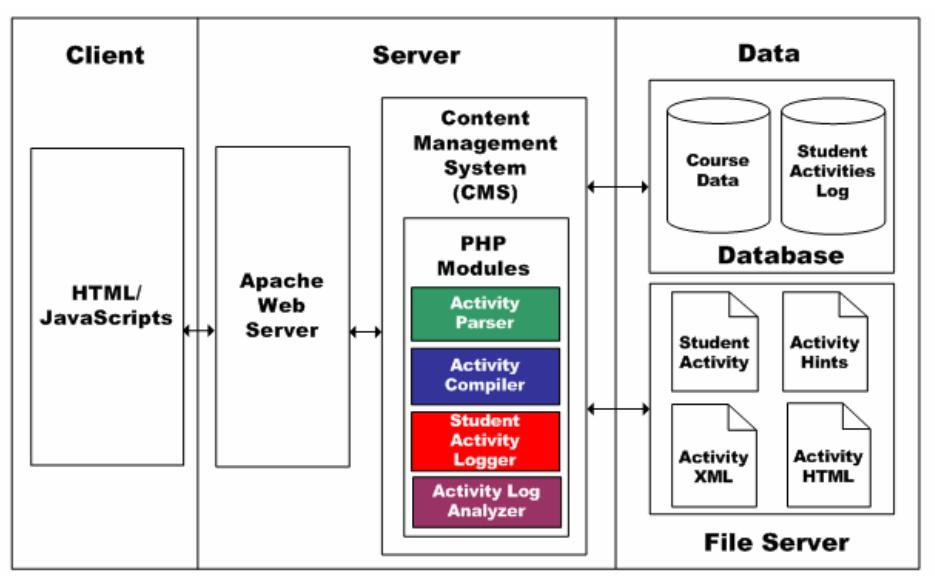
\includegraphics[width=0.9\linewidth, keepaspectratio =
1]{./images/SystemArch01_OUHK_DistanceEdu.jpg}
  \caption{Sistemska arhitektura spletnega portala za učenje
    programiranja, kot so jo naredili na OUHK \cite{ITaLCP_DistanceEdu}.}
  \label{fig:OUHK_cmsArch}
\end{figure}

Ti moduli so naslednji, zajem aktivnosti, prevajalnik aktivnosti,
dnevnik študentove aktivnosti in analizator dnevnikov aktivnosti. Samo
delovanje je naslednje, ko odjemalec pošlje zahtevo za neko aktivnost,
se ta naslovi strežniku, ki poišče programsko aktivnost. Z modulom
\emph{zajema aktivnosti}, strežnik zajame aktivnost, ki je zapisana v
obliki \textbf{XML} in naloži vse potrebne datoteke. Zajem aktivnosti,
prav tako naloži študentovo predhodno delo, ki je shranjeno datoteki
aktivnosti. Ko se vse zajame in naloži se vsebina pošlje v obliki
\textbf{HTML} nazaj k klientu.

Strežnik omogoča tudi prevajanje aktivnosti. Ko strežnik dobi prošnjo
za prevajanje programske kode, se ta prevede, če seveda v njej ni
sintaktičnih napak in se ustvari datoteka \textbf{JAR}, ki jo študent
lahko prenese s strežnika. Če so v programu napake, se ustvari dnevnik
napake, v trenutni aktivnosti, prav tako se napaka izpiše na zaslonu
študenta. Vsako aktivnost zajame dnevnik študentove aktivnosti in jo shrani v
podatkovno bazo. Z analizatorjem dnevnika študentove aktivnosti,
mentorji dobijo vpogled v delo študenta in njegovega napredka.

\subsection{Pregled delovanja in interakcija s SPUP}
\label{sec:pregled_delovanja_in_interakcija}

Opišimo, kako so si zamislili interakcijo med študentom in mentorjev s
spletnim sistemom na \textbf{OUHK}. Diagram prikazuje slika
\ref{fig:OUHK_workFlow}. Spletni sistem omogoča študentom in mentorjem
spletno okolje za učenje programiran. Mentorji na spletni portal
naložijo snov preko spletnega brskalnika. Mentor lahko naloži datoteke
opisom aktivnosti. Ta datoteka vsebuje osnovne opise in informacije o
aktivnostih. Posebej naloži še datoteko v kateri je predloga za
aktivnost. V to predlogo študent rešuje zadano nalogo. V posebno
datoteko je naložen tudi namig, ta je študentu v pomoč in ponuja
primer izpisa programa.

\begin{figure}[htb!] \centering
  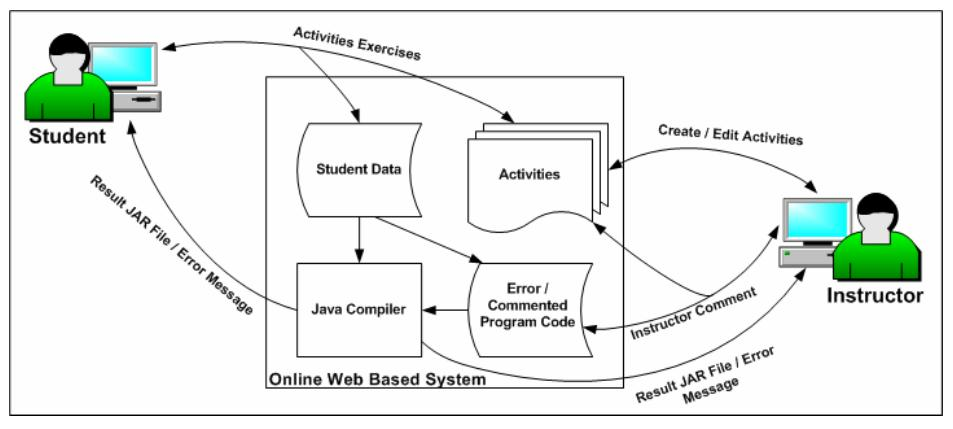
\includegraphics[width=0.9\linewidth, keepaspectratio =
1]{./images/SystemArch02_OUHK_DistanceEdu.jpg}
\caption{Prikaz med interakcijo študenta in mentorja s spletnim
  portalom \cite{ITaLCP_DistanceEdu}.}
  \label{fig:OUHK_workFlow}
\end{figure}

Študent lahko pregleduje vse aktivnosti in si naloži katero koli izmed
njih. Omogočeno ima, da program prevede na strežniku, ko prevajalnik
naleti na napake strežnih vrne napako na spletno stran. Če študent
naleti na težavo, ki je povezana z reševanjem aktivnosti, lahko pošlje
prošnjo za pomoč svojemu mentorju. Ko se mentor prijavi v sistem ima
vpogled v napako in na začasno delovno datoteko študenta, mentor lahko
zaganja prevajalnik na tem začasnem projektu študenta. Ko mentor
popravi programsko napako, odgovori študentu in poda komentar na
programsko kodo študenta. Študent ima vpogled v komentarje in
predloge, ki jih je posredoval mentor \cite{ITaLCP_DistanceEdu}.

%%NJihova diskusija, zaključek in nadaljnjo delo.

Na univerzi v US \cite{mentalModels}, je okrog strategije kognitivnega konflikta
nastalo spletno okolje, ki naj bi izboljšalo mentalne
modele ključnih programskih konceptov. Učni model je sestavljen iz
štirih korakov:

\begin{itemize}
\item \textbf{Predhodni korak:} Mentor razišče kakšni so predhodni
 mentalni modeli študentov in identificira neprimerne.
\item \textbf{Korak kognitivnega konflikta:} V študentovi predstavi
  moramo sprožiti tak dogodek, ki v študentu izove neskladje z njegovo
  predhodno predstavo in s tem študenta potisnemo v konfliktno
  situacijo.
\item \textbf{Korak konstruiranja modela:} Študentu s pomočjo
  visualizacije pomagamo ustvariti pravo mentalno predstavo.
\item \textbf{Korak aplikacije: } Študent mora rešiti programsko
  nalogo z na novo ustvarjeno mentalno predstavo.
\end{itemize}

Spletno učno okolje podpira programski jezik \textbf{JAVA}. Za učenje
programskih konceptov je na spletni strani vsak posamezen koncept
povezan z potjo, ki predstavlja načrt potovanja. Poti koncepte se
povezujejo tako, da se ti nadgrajujejo, saj znanje določenega koncepta
potrebuje neko predznanje prejšnjega. Tako za razumevanje določevanja
reference najprej potrebujemo predznanje o spremenljivkah ali
npr. preden se študenti učijo kako s podajajo parametri v podprograme
najprej morajo razumeti kaj je obseg nekega pod programa. Torej je
vrstni red spoznavanja programskih konceptov pomemben. Med potmi so
gumbi, ki predstavljajo vsak koncept. Na vsakem gumbu je označen rdeč
križ kar pomeni, da študent še ni spoznal koncepta. Ko študent opravi
naloge povezane s posameznim konceptom se rdeč križ spremeni v zeleno
kljukico. Ko študent vstopi v koncept se izpiše študentova zgodovina z
nalogami tega koncepta. Vsaka naloga vsebuje tako vprašanje, ki sproži
konfliktno situacijo v mentalnem modelu študenta. Nato študenti dobijo
učni material v visualni obliki. Za vizualizacijo uporabljajo orodje
\href{https://cs.joensuu.fi/jeliot/}{\textbf{Jeliot}}, ki dinamično
upodablja izvajanje javaskih programov. Za pravilnost razumevanje
mentalnega modela mora študent odgovoriti na dodatna vprašanja. Če
študentovi odgovori niso v skladu z podanim mentalnim modelom, dobi
študent povratno informacijo o nepravilnem odgovoru. Naslednji korak
je ta, da študent mora zagnati vizualizavijo dela programske kode, ki
si ga je prej moral predstavljati. Tako ima možnost, da zazna
nepravilnost v svojem mišljenju in tako lahko gradi na pravilnem
konceptu \cite{mentalModels}.

%% QUTA
V preteklosti je bilo razvitih mnogo orodij, ki so nastala ravno z
raziskovanja učenja programiranja, vendar mnoga od teh zahtevajo, da
študenti pišejo celotne programe od začetka do konca. Spletni portal
v primeru QUTA uči programiranja v programskem jeziku Java in ima
naslednjo naslednje zmožnosti \cite{thesisAWebP}.

\begin{enumerate}
\tightlist
\item Spletni portal za programiranja, ki omogoča naloge tipa ``Zapolni
   prazna mesta''.
 \item Ogrodje za analizo, ki preverja kvaliteto in pravilnost, nalog,
   tipa "Zapolni prazna mesta".
 \item  Avtomatski sistem za dajanje povratnih informacij, ki sporoča
   prilagojena sporočila prevajalnika in formalni odziv študentom in
   njihovim mentorjem. Poročilo vsebuje kvaliteto napisanega programa,
   strukturo in pravilnost glede na programsko analizo.
\end{enumerate}

\subsection{Rezultati izvedenih rešitev SPUP}
\label{sec:rezultati_izvedenih_rešitev}

Večina študentov smeri računalništva na OUHK nima predhodnih izkušenj
v programiranju z programskim jezikom \textbf{JAVA}. Sistem se
uporablja kot spletno okolje za učenje programiranja. Študentom je s
tem, dana množica aktivnosti oz. nalog, katere morajo sami uspešno
opraviti. To lahko počnejo kadarkoli in od koderkoli. Študentom ni
potrebno nastavljati programskega okolja, študenti vse programe, ki
jih napišejo, lahko takoj prevedejo in jih zaganjajo na svojih
računalnikih. Uporaba spletnega portala je pokazala da so študentje
oddali 100\% programskih nalog, napisanih v javi. To kaže na to, da so
študentje samozavestno reševali naloge in jih oddajali. Pred uporabo
spletnega portala je oddaja nalog bila 80\%.

Kot pravijo avtorji članka in portala \cite{ITaLCP_DistanceEdu}, je to
šele začetek uporabe spletnega portala, ki nudi osnovno
funkcionalnost. V nadaljevanju nameravajo dodati še inteligentni
sistem, ki po nadzoroval napredek študentov.

Za izboljšanje mentalnih modelov so avtorji predlagajo konstruktivno
naravna učni model, ki vključuje strategijo kognitivnega konflikta in
vizualiacijo programov. Zgodnje preizkušanje strategije kognitivnega
konflikta pokažejo da so študenti bolj zavzeti za učni material in jih
motivira tako, da si prej ustvarijo pravilno mentalno predstavo
\cite{mentalModels}.

Tudi začetniki, ki uspešno premagajo začetne ovire in se lotijo
takojšnjega programiranja, imajo zelo slabo napisano in konstruirano
programsko kodo. Pomagati novincem, pistati kvalitetno programsko kodo
je časovno zelo zahtevno opravilo.

%Danes se večini uči OO jezikov, kako podkrepiti to tezo.
Težave programiranja se stopnjujejo ko se za učenje programiranja
uporabljajo Objektno-orjentirani programski jeziki, sej ti zahtevajo
visoko stopnjo abstraktnega razumevanja programskih konceptov in so
načrtovani predvsem za zahtevne programerje.

% Torej je pomembno v katerih programskih jezikih se začnemo učiti
% programiranja? Zakaj sta zato primerna? -> Scratch in Python?  Kje
% je določeno na državnem nivoju da se učit ravno ta dva programska
% jezika

Rezultat dela avtorjev spletnega portala QUTA, gre še nekoliko naprej
od OUHK in v njihov spletni portal vgradijo, odziv spletnega portala,
ki mora o pravilnosti programa in o kvaliteti. Ogrodje
\emph{(ang. framework)} za analizo programske kode vsebuje naslednje
komponente \cite{thesisAWebP}.

\begin{itemize}
\tightlist
\item
  Sintaktično ali semantično opozarjanje na napake ali napake
  prevajalnika.
\item
  odziv na kvaliteto in pravilnost programske kode.
\item
  Formalni odzin učitelja oz. komunikacija med učiteljem in učencem.
\end{itemize}

\subsection{Značilnosti SPUP}
\label{sec:značilnosti_spup}

Ena od osnovnih in glavnih komponent pri vseh SPUP je orodje, ki
omogoča pisanje in preizkušanje programske kode. Poimenujemo jo lahko
kot \textbf{Spletna aplikacija za programiranje}. Njene
glavne značilnosti so naslednje:

\begin{itemize}
  \item \textbf{urejevalnik besedil}, ki ima lahko osnovne funkcije ali tudi
  zahtevne, ki so značilne za \textbf{IDE};
\item omogočen je zagon napisanega progama z vhodnimi in izhodnimi
  podatki;
\item omogočena je \textbf{povratna informacija}:
  \begin{itemize}
    \tightlist
  \item \textbf{sintaktičnih napak}, ki ju vrne prevajalnik ali tolmač;
  \item \textbf{semantičnih napak}, ki preverjajo željen rezultat napisanega
    programa oz. pravilno rešitev;
  \end{itemize}
\end{itemize}

Iz pregleda SPUP, ki so nastali na univerzah smo se lahko poučili, kaj
so nekatere značilnosti spletnih portalov. Strnimo te značilnosti, saj
jih bomo pozneje uporabili pri iskanji, kategoriziranju in
vrednotenju.

Spletni portal vsebuje:

\begin{itemize}
\tightlist
\item razdelano vsebino z nalogami oz. aktivnostmi;
\item \textbf{Spletno aplikacijo za pisanje programske kode};
\item omogočena je komunikacija med mentorjem in novincem;
\item omogočen je pregled nad napredkom novincem oz. tako imenovan
  \emph{nadzor nad razredom}.
\end{itemize}

\section{Strategije pouka}
\label{sec:didaktika_racunalnistva}


% To še točno ne vem kam bi dal
% Primer strategij in metod spletnega portala za učenje \textbf{Jave}.
% \cite{thesisAWebP}:

% \begin{itemize}
% \tightlist
% \item
%   Scaffolding -\textgreater{} Gradnja študentovega znanja
%   pri katerem pomaga mentorja, z svojim znanjem in izkušnjami.
% \item
%   Bloomova taskonomija. Zakaj je pomembno vključevanje Bloomove
%   taksonomije in kako jo vključujemo.
% \item
%   Konstruktivizem: Aktivnost študentov pri gradnji znanja. Učenje z
%   eksperimentiranjem. Problemski pristop.
% \end{itemize}

% Kaj od katerih metod predstavlja v uporabi spletnega portala \ldots{}:

% \begin{itemize}
% \tightlist
% \item
%   Spletni portal -\textgreater{} Scaffolding + Bloom
% \item
%   Naloge narejene tako, da podpirajo konstrutivno metoIn tudi nekatere slabosti, če hih najdem v literaturi
%   -\textgreater{} problemski pristopom
% \end{itemize}

% V naslednjem poglavju sledi pregled tehnik aktivnih metod
% poučevanja. V poglavju sledi obravnava didaktičnih pripomočkov, oblik
% pouka, in projektno delo \cite{guideTCS}.

\subsection{Aktivno učenje in model aktivnega učenja}
\label{sec:aktivno_učenje_in_model_aktivnega_učenja}

Vsak pouk računalništva mora biti zgrajen kot model in bi moral
upoštevati naslednja načela:
\begin{itemize}
\tightlist
\item Vzpodbujati mora študente z pozitivno naravnanim poukum in
   omogočati mora okolje kjer študent najde pomoč.
 \item Pouk računalništva je grajen na konstruktivnih metodah poučevanja
   in aktivnem učenju.
\end{itemize}

\textbf{Konstruktivizem} je kognitivna teorija, ki preučuje naravo
procesov učenja. Po tem principu naj bi učenci konstruirali novo
znanje na osnovi preurejanja in izpopolnjevanja že obstoječega
znanja. Znanje se gradi na obstoječih mentalnih strukturah in na
odzivu, ki ga dobi učenec iz učnega okolja. Mentalne strukture so
grajene korak za korakom, ena za drugo, seveda s to metodo lahko pride
tudi do sestopanja ali slepih koncev. Proces je povezan z Piagetovim
mehanizmom asimilacije \cite{guideTCS}.

Pri \textbf{aktivnem učenju} je najpomembnejše to, da učenci z lastno
aktivnostjo ugotovijo, sami za sebe kako nekaj deluje. Sami si morajo
izmisliti primere, preiskusiti lastne veščine in reševati neloge, ki
so jih že ali jih še podo spoznali. Učenje je aktivno usvajanje, je
gradnja idej in znanja. Za učenje mora biti posameznik aktivno
vključen v gradnjo svojih lastnih mentalnih modelov.

Model aktivnega učenja je sestavljen s štirih korakov \cite{guideTCS}.

\begin{itemize}
\tightlist
\item \textbf{Sprožilec} Je je naloga, ki predstavlja  iziv za uvod v novo
tematiko.  //Gerlič -> Motivacija.
\item \textbf{aktivnost} Študenti izvajajo aktivnost, ki jim je bila
predstavljena v sprožilcu. Ta kora je lahko kratek ali lahko
zavzame večju del učne ure. To je odviso od vrste sprožilca in
izobraževalnih ciljev.
\item \textbf{diskusija} sledi po koncu aktivnosti, kjer se zbere zeloten
razred, neglede na obliko dela. V temo koraku študenti izpopolnijo
koncepte in ideje, kod del konstruktivnega učnega procesa.
\item \textbf{povzetek} je lahko izračen v različnih oblikah, kot so
zaogrožene definicije, lahko so miselni vzorci ali povezav med
temami, ki so jih obravnavali študenti in med drugimi temami, ki se
navezujejo nanje.
\end{itemize}

Ko se ta model izkaže za primernega, ga lahko uporabimo v številnih
učnih urah v različnih variacijah.


\subsection{Strategije reševanja problemov}
\label{sec:strategije_reševanja_problemov}

Programiranje je preces pri katerem rešujemo probleme. Reševanje
problemov, zato mora biti središče poučevanja računalniške
znanosti. Reševanje problemov je zahteven mentalni proces. Če na
spletu pobrskamo za strategije reševanja problemov lahko hitro
ugotovimo na obstajajo različne strategije. Kot so recimo naštete na
strani
\href{https://en.wikipedia.org/wiki/Problem_solving#Problem-solving_strategies}{Wikipedia:Reševanje
  problemov (\emph{ang. Problem solving})}, abstrakcija, analogija,
brainstorming, deli in vladaj in mnoge druge.  Proces in tehnike
reševanje problemov se uporablja v mnogih tehničnih in znanstvenih
disciplinah \cite{guideTCS}.

V nekaterih primerih učenci sami razvijejo strategijo s katero rešijo
nek problem. Otroci si na primer sami izmislijo enostvno seštevanje in
odštevanje, dolgo pred tem kadar se to učijo pri pouku
matematike. Toda brez formalne podpore za unčikovito strategijo
reševanja problemov, spodleti še tako inovativnemu učencu tudi pri
enostavnih strategijah kot je \textbf{preizkus in napaka}. Zato je
pomembno, da se uči strategij za reševanje problemov.

%\subsection{Proces reševanja problemov}
%\label{sec:proces_reševanja_problemov}

Vsak osnoven proces, ki se ukvarja z raševanjem problemov, ne glede na
znanstveno disciplino, se začne z opisom problema. Vsak problem se
navadno zaključi z neko rešitvijo, ki je v nekaterih primerih izražena
z \textbf{zaporedjem korakov} ali \textbf{algoritmom}. V računalništve
algoritem zapišemo z kodo nekega programskega jezika. Zapisan
algoritem testiramo tako, da kodo zaženemo, jo izvedemo. Preden
pridemo od opisa problema do podane rešitve moramo prehoditi kar nekaj
težkih korakov. Na te vmesne korake lahko gledamo kot na procese
odkrivanja, zato lahko na reševanje problemov gledamo tudi kot na
kreativen, umetniški proces Splošno priznani koraki reševanja procesov
so naslednji \cite{guideTCS}:

\begin{enumerate}
\tightlist
\item \emph{Analiza problema}. Najprej je pomembno da razuemo kaj je
  problem in ga znamo identificirati. Če tega ne znamo, ne moremo
  priti do nobene rešitve.
\item \emph{Alternativnie rešitve}. Razmišljamo o alternativnih
  rešitvah kako bi lahko rešili nek problem.
\item \emph{Izbira pristopa}. Izberemo primeren pristop, kako rešiti problem.
\item \emph{Razgradnja problema}. Problem razgradimo na manjše podprobleme.
\item \emph{Razvoj algoritma}. Algoritem razvijamo po korakih, ki smo
  jih določili v podproblemih.
\item \emph{Pravilnost algoritma}. Preverjanje pravilnosti algoritma.
\item \emph{Učinkovitost algoritma}. Izračunamo učinkovitost algoritma.
\item \emph{Refleksija}. Naredimo refleksijo in analizo na pot, ki smo
  jo naredili pri reševanju problema in naredimo zaključek z tem kar
  lahko izboljšamo za naslednji problem, ki ga bomo reševali.
\end{enumerate}

Točen recept kako se lotiti reševanja ne obstaja. Učencem lahko le
pokažemo nekatere metode in strategije, ki jim lahko pomagajo pri
reševanju problemov. Poglejmo še nekatere pomembne korake podrobneje.

\subsubsection{Razumevaje problema}
\label{sec:razumevanje problema}

Razumevanje problemov je prva stopnja v procesu reševanja
problemov. Pri reševanju algoritemskih nalog najprej moramo
prepoznati, kaj so vhodni podatki in kateri podatki naj bi bili
izhodni. Če znamo povedati kaj bodo vhodni podatki, razumemo tudi
bistvo samega problema.

\subsubsection{Načrtovanje rešitve}
\label{sec:načrtovanje_rešitve}

Novinci se spopadajo z največjimi težavami na začetni stopnji
načrtovanja rešitve za nek problem. V nadaljevanju so predstavljene
tri strategije, ki jih lahko uporabimo na tem koraku reševanja
problema.

\begin{description}
\item [Definicija spremenljivk problema:] Pri rešitvi problema
  si pomagamo tako, da ugotovimo kaj morajo biti vhodni in kateri bojo
  izhodni podatki. S tem razjasnimo problem. V naslednjem koraku
  definiramo \textbf{spremenljivke}, ki so potrebne za rešitev
  problema.
\item [Postopno izboljševanje (\emph{ang. Stepwise
      Refinement)}:]Po tej metodi nas najprej zanima celoten pregled
  strukture problema in odnosi med posameznimi deli. Zatem se šele
  poglobimo specifični in kompleksni implementaciji posameznih pod
  problemov. Postopno izboljševanje je metodologija, ki poteka od
  \textbf{zgoraj-navzdol}, torej od splošnega k specifičnemu. Drugačen
  pristop je od \textbf{spodaj-navzgor}. Za oba pristopa velja da eden
  drugega dopolnjujeta. V obeh primerih je problem razdeljen na manjše
  pod probleme ali naloge. Glavna razlika med obema je mentalni
  proces, ki je potreben za en ali drugi pristop.  V nadaljevanju se
  posvetimo samo pristopu od \textbf{zgoraj-navzdol}. Rešitev, ki jo
  poda \textbf{postopno izboljševanje} ima modularno obliko, ki jo:
  \begin{enumerate}
    \tightlist
  \item jo lažje razvijamo in preverjamo,
  \item jo lažje beremo in
  \item nam omogoča, da uporabljamo posamezne pod rešitve tudi za
    reševanje drugih problemov.
  \end{enumerate}
\item [Algoritemski vzorci:] Algoritemski vzorci združujejo
  matematični pogled in elemente načrtovanja. Vzorec podaja načrt na
  rešitev, s katero se srečamo mnogokrat. Algoritemski vzorci so
  primeri elegantnih in učinkovitih rešitev problemov in predstavljajo
  abstraktni model algoritemskega procesa, katerega lahko prilagodimo
  in ga integriramo v rešitve drugim problemom.

  Pri tem procesu lahko nastopi težava prepoznave vzorca algoritma pri
  novincih, saj ti niso sposobni prepoznati podobnosti med posameznimi
  algoritmi ali ne znajo prepoznati bistvo problema, njihove posamezne
  komponente in razmerja med njimi, da bi lahko rešili nove
  probleme. V takih primerih novinci radi ponovno izumijo že njim
  poznane rešitve, ki bi jih lahko uporabili. Te težave navadno
  nastanejo zaradi slabe organizacije sistematike znanja o algoritmih.

  Proces reševanja problemov z algoritemskim vzorcem se navadno začne
  z prepoznavanjem komponent, ki vodijo k rešitvi in iskanjem podobnih
  problemov, na katere še imamo znane rešitve. Zatem prilagodimo
  vzorec prilagodimo za rešitev problema in ga vstavimo v celotno
  rešitev. V večini primerov je potrebno vstaviti več različnih
  vzorcev, da dobimo neko novo rešitev.
\end{description}

\subsubsection{Preverjanje rešitve}
\label{sec:preverjanje_rešitve}
Ko imamo pripravljeno rešitev moramo preveriti ali je ta
pravilna. Pogled na preverjanje pravilnosti rešitve je lahko
teoretične in praktične narave. Razhroščevanje (\emph{ang. debugging})
spada me vrsto aktivnosti, ki nam pomaga pri ugotavljanju pravilnosti
rešitve. Splošno velja da proces razhroščevanja, z programom, ki nam
pomaga razhroščevati (ang. debugger) ali brez njega, poglablja
razumevanje računalniške znanosti. Z tem ko učenci razmišljajo, kako
bodo preverjali ali njihov program deluje pravilno, hkrati v njih
poteka miselni proces refleksije o tem kako so implementirali določen
program in kako ga bojo morebiti morali spremeniti.

Na nivoju do srednje šole uporabljamo praktične metode ugotavljanja
pravilnosti programa, kot je razgroščevanje. Ko želimo znanje
pravilnosti delovanja poglobiti se lahko lotimo tudi teoretične
analize.

\subsubsection{Refleksija}
\label{sec:refleksije}

Refleksija je mentalni proces ali obnašanje, ki nam omogoča da neko
delovanje analiziramo in o njem tudi premislimo. Refleksija je
pomembno orodje v splošnem učnem procesu, prav tako spadam med
kognitivne procese višjega reda. Z refleksijo učenec dobi priložnost,
da stopi korak nižje in premisli o svojem razmišljanju in tako
izboljša veščino reševanja problemov. Refleksivno razmišljanje je
proces, ki zahteva veliko časa in vaje. Med procesom reševanja
problemov, lahko refleksijo uporabimo na različnih stopnjah.

\begin{itemize}
\tightlist
\item \emph{Pred} reševanjem problemom. Ko problem preberemo, in že
  načrtujemo rešitev, se splača uporabiti refleksijo in razmisliti o
  tem ali smo morda že reševali podoben problem in temu primeren
  vzorec algoritma.
\item \emph{Med} reševanjem problema. Ko rešujemo problem refleksija
  služi, kot pregled, kontrola in nadzor. Na primer, ko nastopijo
  težave pri načrtovanju rešitve ali morda zaznamo težavo ali
  napako. Temo procesu lahko pravimo \textbf{refleksija v akciji}.
\item \emph{Po} reševanju problema. Ko že najdemo rešitev, ki deluje,
  nam refleksija služi kot orodje z katerim pregledamo učinkovitost
  delovanja. Pregledamo strateške odločitve, ki so bile sprejete med
  samim načrtovanjem rešitve.
\end{itemize}

Refleksija je kreativni proces in je pomemben za učenca tako kot za
učitelja.

\subsection{Programirana pouk}
\label{programirani_pouk}




\subsection{Projektno delo}
\label{sec:projektno_delo}

Preglejmo najprej nekatere lastnosti, ki jih prinaša projektno
delo. To lahko poteka tako, da učenci delajo samostojno ali v
skupini. Učitelj je tisti, ki vodi proces projektnega dela. Učenec je
pri projektnem delu bistveni člen in mu tako omogoča aktivno učenje.


\subsection{Učenje  na daljavo}
\label{sec:Učenje_na_daljavo}

%%Od tu naprej je nova datoteka pregled.tex

%%% Local Variables:
%%% mode: latex
%%% TeX-master: "diploma"
%%% End:

\newpage
\section{Kriteriji za klasifikacijo spletnih portalov}
\label{sec:kriteriji_za_klasifikacijo_spletnih_portalov}

Spletni portali imajo različne značilnosti in zmožnost. V poglavju
bomo razdelali posamezne kriterije s katerimi bomo klasificirali in
ovrednotili posamezne spletne portale.

\subsection{Vrsta vsebine}
\label{sec:Razvrstitev_spletnih_portalov}

Po hitrem pregledu in iskanju spletnih portalov lahko ugotovimo, da
spletni portalu za učenje programiranja ponujajo najrazličnejše vrste
vsebin in njihove kombinacije kot je na primer, \textbf{tekstovni
  vodič in spletno aplikacija za programiranje}. V posebno kategorijo
bomo uvrstili tudi spletne portale, ki ponujajo \textbf{spletne igre},
ki učijo programiranje. Različne vrste spletnih portalov, ki jih lahko
obravnavamo so naslednje:

\begin{itemize}
\tightlist
\item \textbf{tekstovni vodič}i,
\item \textbf{video vodič},

\item \textbf{spletna aplikacija za programiranje}, kot smo jo
  definirali v poglavju \ref{sec:značilnosti_spup},
\item \textbf{spletne igre},
\item \textbf{kombinacija} vrst vsebin, ki jih lahko še razdelimo na:
  \begin{itemize}
    \tightlist
  \item \textbf{najosnovnejša kombinacija} (\emph{tekstovni vodič + preizkus kode});
  \item \textbf{napredna kombinacija} (\emph{različne vrste vodičev +
      spletna aplikacija za programiranje}).
  \end{itemize}
\end{itemize}

V tej diplomi se ne bomo specifično ukvarjali s tem katera izmed vrst
vsebin predstavlja boljše zmožnosti za prenos znanja. Vsaka ima svoje
prednosti in slabosti, zato bomo za vsako izpostavili njene pozitivne
značilnosti tudi slabosti. Zanimale nas bodo predvsem tise
\textbf{kombinirane} vrste vsebin, ki bodo predstavljale čim bolj
celovit spletni portal za učenje programiranja, kot smo ga definirali
v poglavju \ref{sec:značilnosti_spup}.

%Kje naredim razdelek med spletnim portalom z vsebino in tistim, ki
%ponuja razvojno okolje in služi le kot orodje za preizkus programske
%kode in potrebuje da učitelj sam doda vsebino.

\subsubsection{Tekstovni vodiči}

Spletni vodiči so najstarejša metoda podajanja znanja. Spletni vodiči
imajo značilnost, da uporabnika vodijo \textbf{po koraki}h do nekega
določenega cilja. Besedilo, ki podaja znanje je opremljeno z
\textbf{primeri}. \cite{wiki:tutorials}

Značilni predstavniki takih vodičev je spletna stran
\url{https://docs.python.org} na kateri najdemo vso dokumentacijo
programskega jezika \textbf{Python}. Na strani najdemo tudi vodiča z
naslovom \emph{\href{https://docs.python.org/3/tutorial/index.html}{The
  Python Tutorial}} \cite{web:TPythonTut The}.

\begin{figure}[h!]
    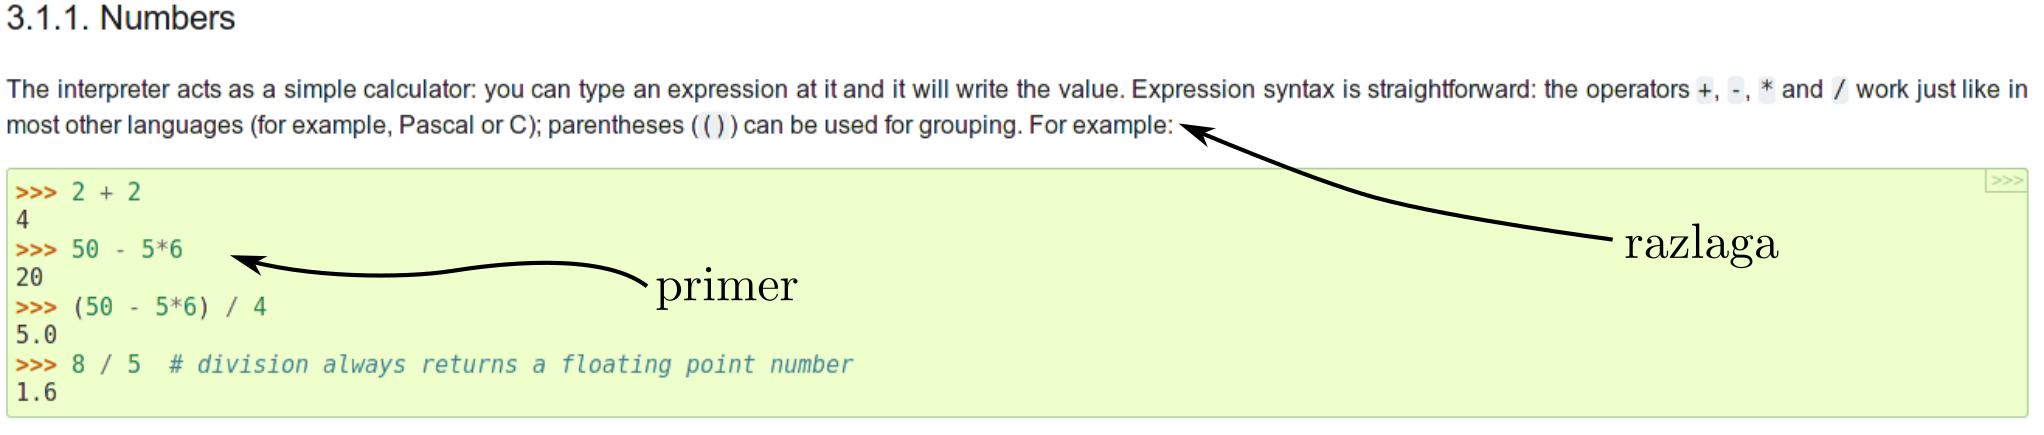
\includegraphics [width=1\linewidth, keepaspectratio =
    1] {./images/sc_web/tPyTut_01.png}
    \caption{Zaslonski posnetke poglavja z vodiča
      \emph{\href{https://docs.python.org/3/tutorial/index.html}{The
          Python Tutorial}} s primerom \cite{web:TPythonTut}.}
    \label{fig:scr:web:tPyTut}
\end{figure}

Spletne vodiče pri pouku uporabljamo na podoben način kot pri
\textbf{metodo dela s tekstom}. Sicer je pomembno da učenci usvojijo
uporabo spletnih vodičev, vendar so spletni vodiči marsikdaj
prezahtevni za uporabo sploh na osnovno šolskem nivoju. Negativna
stran spletnih vodičev je še ta, da direktno s spletne strani ne
moramo preizkušati primerov programske kode, kar je slabo tudi Z
motivacijskega vidika.

\subsubsection{Video vodiči}
\label{sec:video_vodici}

Z razmakom video vsebin na spletu, so marsikateri spletni vodič
dopolnili oz. zamenjali video vodiči. Popularno je postalo zajemanje
oz. \textbf{snemanje lastnega namizja}. Vido vodiče najdemo za
številna področja, od uporabe določene programske opreme in vse do
programiranja. Ena izmed prednosti video vodičev naprem tekstovnim je
ta, da ti omogočajo nazornejši prikaz nekega postopka. Preden sami
posnamemo nek postopek, lahko v video posnetku opazujemo vsak korak,
potek miške in poleg teka poslušamo razlago, če je ta vključena.
Številne študije kažejo da je učenje s multimedijo, torej kombinacijo
zvoka in slike dosti bolj učinkovito, samo poslušanje ali branje
teksta \cite{web:multimediaL}. V razredu je uporaba video vodičev
lahko koristna pri samostojnem delu in domačem delu. Uporaba video
vodičev ima tudi slabe strani, v njih lahko predstavimo dosti manj
vsebine in iskanje vsebine ni preprosto, kot je to pri tekstu.

Eden izmed spletnih portalov, ki je specializiran za podajanje znanja
s video vodiči je \emph{\href{https://www.udemy.com}{Udemy}}
\cite{web:udemy}. Na njem vsak kdo lahko postane učitelj in pripravi
učne ure z različnih področij, ne samo z računalniške
znanosti. Nekateri sklopi učnih ur so v celoti brezplačni, večin je
plačljivih.

\begin{figure}[h!]
    
\includegraphics [width=1\linewidth, keepaspectratio =
    1] {./images/sc_web/udemy_01.png}
    \caption{Zaslonska slika spletne strani
      \emph{\href{https://www.udemy.com}{Udemy}}
      \cite{web:udemy}. Na prosto dostopnem sklopu učne ure v
      pythonu.}
    \label{fig:scr:web:udemy}
\end{figure}

\subsubsection{Spletna aplikacija za programiranje.}
\label{sec:spletna_app_programiranje}

Nekatere spletne strani ponujajo le spletno aplikacijo za
programiranje, kot smo jo povzeli v poglavju
\ref{sec:značilnosti_spup}. Taki spletni portali ne ponujajo vsebine,
ponujajo le \textbf{orodje}. Ali pa ponujajo le toliko vsebine, kot je
potrebno, da se uporabnik nauči uporabljati spletno aplikacijo. Kljub
temu, da nas zanimajo celoviti spletni portali, ki ponujajo tudi
vsebino, nas bodo podrobneje zanimala tudi orodja. Prednost uporabe
spletne aplikacij ali orodja je ta, da ima mentor (\emph{učitelj})
svobodno izbiro, katero vsebino bo podajal. Priprava vsebine sicer
terja več truda in časa mentorja, vendar lahko vsebino prilagaja in jo
prireja po potrebi.

Predstavnik takega orodja je
\emph{\href{http://pythonfiddle.com/}{Python Fiddle}}
\cite{web:pythonfiddle}. Omogoča osnovni urejevalnik besedila (slika), z
barvanjem programske kode, s predlogami za samo dokončevanja izpisa
vgrajenih funkcij. Uvozimo lahko datoteke in jih delimo. Zaganjamo
napisane programe, izhodni podatki se izpišejo v konzoli.

\begin{figure}[h!]
    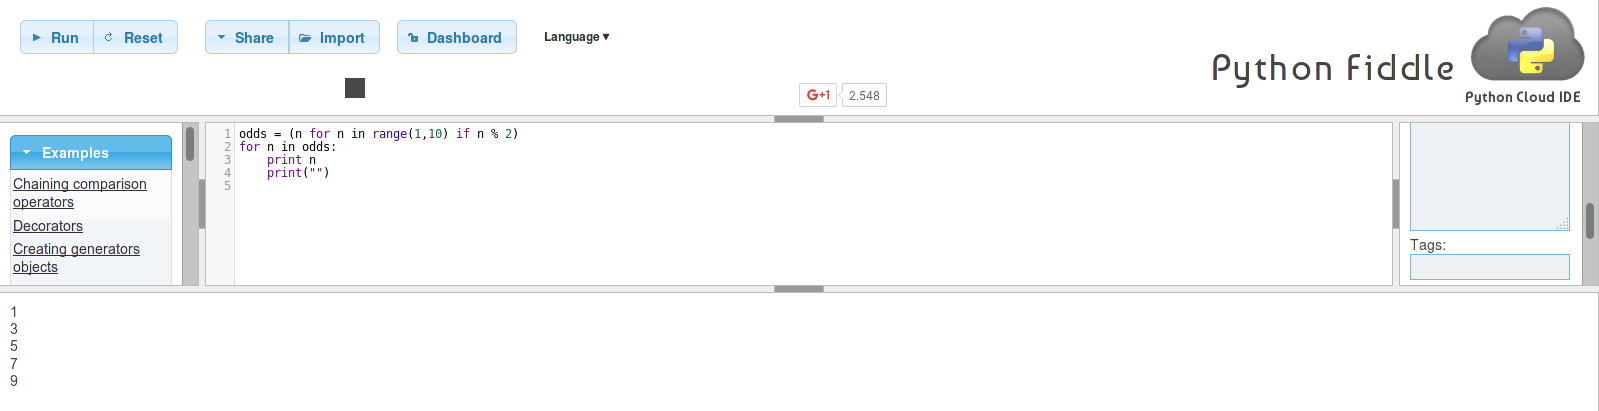
\includegraphics [width=1\linewidth, keepaspectratio =
    1] {./images/sc_web/PythonFiddle_01.png}
    \caption{Zaslonska slika spletne applikacije za programiranje
      \emph{\href{http://pythonfiddle.com/}{Python Foddle}}
      \cite{web:pythonfiddle}.}
    \label{fig:scr:web:PyFiddle}
\end{figure}

Spletne tehnologije so danes zalo napredovale in že nekaj let se
aplikacije in podatki selijo v \textbf{oblak}. Te aplikacije in
podatki so dostopni od koder koli. V \textbf{oblaku} so razvijajo
številna profesionalna okolja \textbf{IDE}, ki omogočajo delo na
večjih projektih in ponujajo napredne funkcije IDE, ki smo jih drugače
lahko imeli le z namiznimi aplikacijami. Navedimo dva primera:
\emph{\href{https://codenvy.com/}{Codenvy}} \cite{web:codeenvy} in
\emph{\href{https://c9.io/}{Cloud9}}\cite{web:cloud9}. Oba ponujata
profesionalen IDE v oblaku. Za uporabo v šoli sta ti dve okolji preveč
zahtevni, in jih ni smiselno uporabljati pri poučevanju novincev. S
tem jim otežimo učenje programiranja, saj prej potrebujejo čas, da
spoznajo in se naučijo uporabljati IDE.

\subsubsection{Spletne igre}
\label{sec:spletne_igre}

Na spletu obstajajo številni spletni portali, ki učijo in spodbujajo k
učenju programiranja s igrami podobnimi vsebinami. Vsebina je
razdeljena na stopnje. Igralci na napreduje iz stopnje v stopnjo in
pri tem nabirajo izkušnje, nove veščine in dosežke. Za igranje igre ne
upravljamo z liki v igri z tipkovnico in miško temveč pišemo
programsko kodo, ki upravlja njihovo početje. Takšni spletni portali
dajejo zelo dobro motivacijsko osnovo, saj se novinci spoznajo na
osnovne principe igranja iger. Primer spletnega portala je
\emph{\href{http://fightcodegame.com/}{Fightcode}}
\cite{web:fightcode}. Igralci programirajo robota v programskem jeziku
JavaScript. Vsak izmed igralcev lahko izzove drugega igralca v boj med
roboti. Za vsako zmago se igralec pomika navzgor po lestvici
najboljših robotov.

\begin{figure}[h!]
    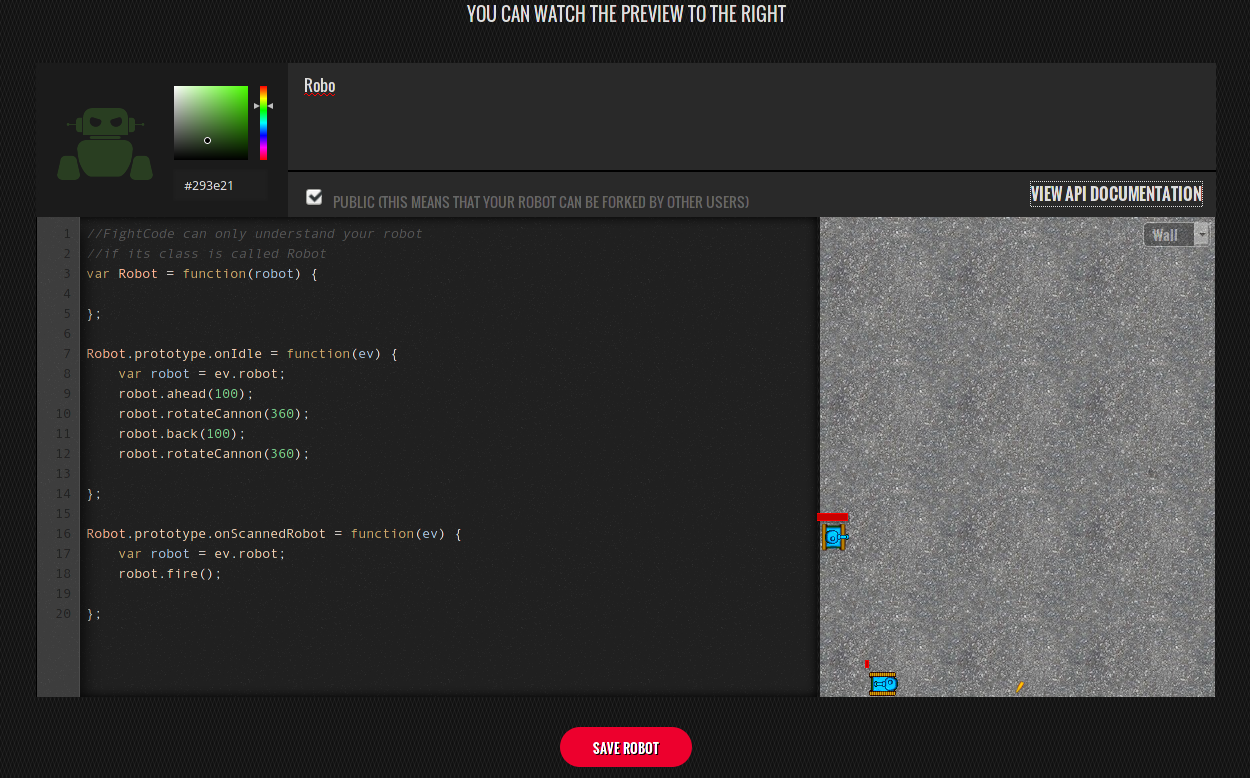
\includegraphics [width=1\linewidth, keepaspectratio =
    1] {./images/sc_web/fightRobot_01.png}
    \caption{Zaslonska slika spletne strani
      {\href{http://fightcodegame.com/}{Fightcode}}
      \cite{web:fightcode}.}
    \label{fig:scr:web:w3school}
\end{figure}

V podrobnem pregledu si bomo še podrobneje ogledali nekatere druge
spletne igre, ki učijo programirati.

\subsubsection{Kombinirane vrste vsebin}
\label{sec:kombinirane_vrste_vsebin}

V prejšnjih poglavjih smo opisali \textbf{osnove vrste} spletnih
portalov. Zanimale nas bodo predvsem \textbf{kombinirane vrste}, ki so
sestavljene iz osnovnih. Te bodo podale celovite portale. Na spletu
najdemo številne kombinacije spletnih portalov,\textbf{Osnovno
  kombinirano vsebino} predstavljajo spletni portali, kot je
\emph{\href{http://www.w3schools.com/}{w3School}}
\cite{web:w3school}. Sestavljeni so iz \textbf{tekstovnih vodičev} in
\textbf{najosnovnejšega preizkusa programske kode}. Vsak primer v
vodiču je opremljen s primerom, katerega lahko zaženemo in preizkusimo
kaj je rezultat primera. Za izvajanje primera pritisnemo na gumb
\textbf{Preizkusi!  (\emph{ang. Try it!})} Programsko kodo primera
lahko tudi spreminjamo in jo ponovno izvajamo.

\begin{figure}[h!]
    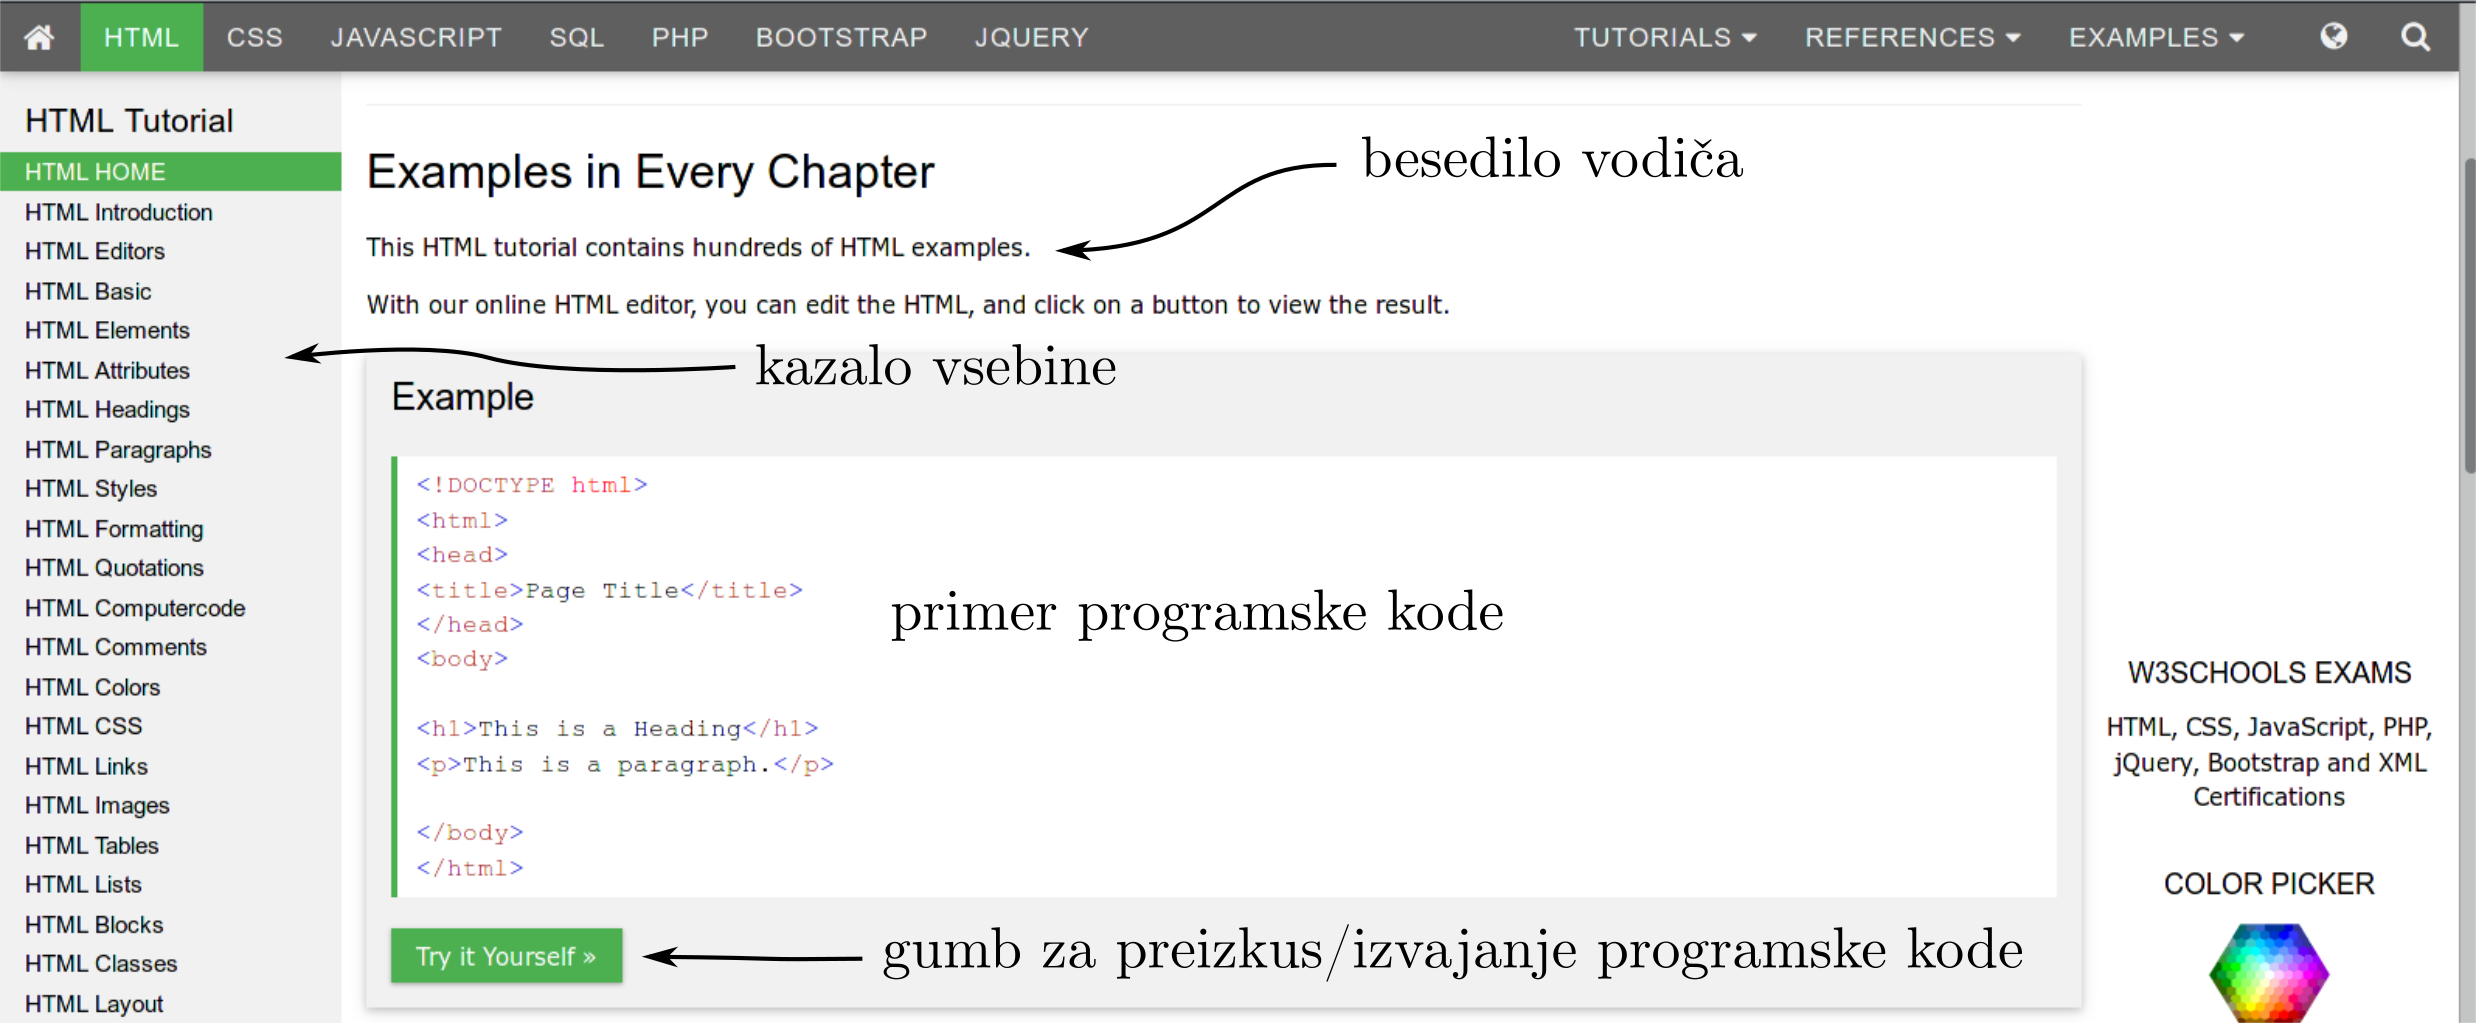
\includegraphics [width=1\linewidth, keepaspectratio =
    1] {./images/sc_web/w3school.png}
    \caption{Zaslonska slika spletne strani
      \emph{\href{http://www.w3schools.com/}{w3School}}
      \cite{web:w3school}.}
    \label{fig:scr:web:w3school}
\end{figure}

\textbf{Napredno kombinirano vsebino} predstavljajo spletni portali, ki so
sestavljeni \textbf{tekstovnega vodiča in/ali video vodičev ter
  spletne aplikacije za programiranje}. Omenimo naslednjega
predstavnika \emph{\href{https://www.codeschool.com/}{Codeschool}}
\cite{web:codeschool}.

\begin{figure}[h!]
    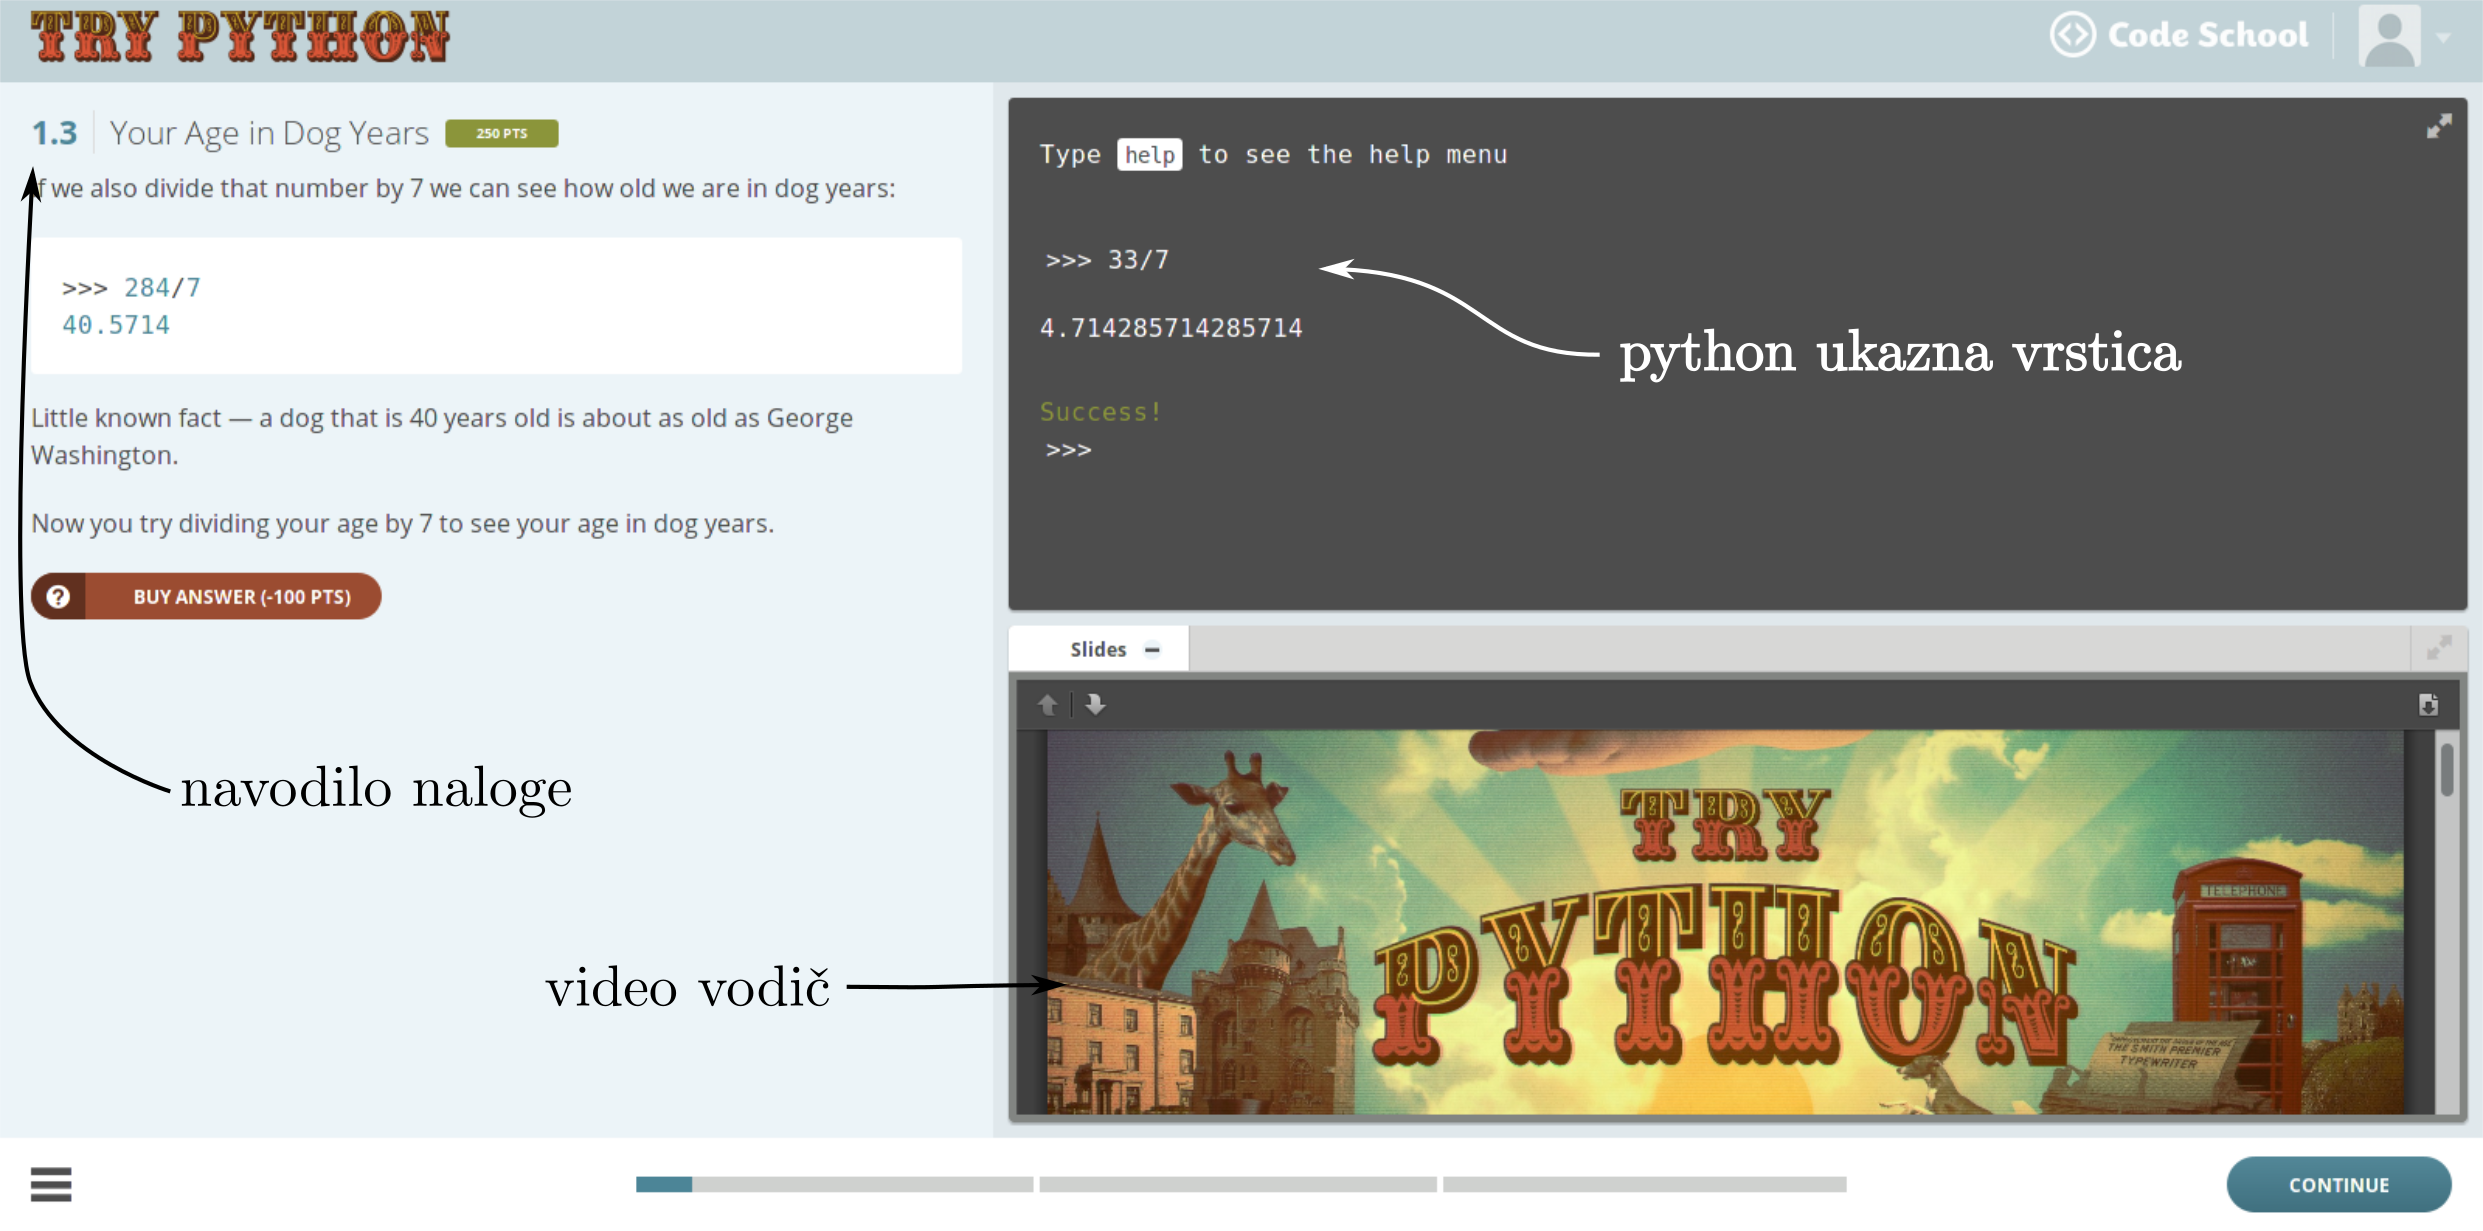
\includegraphics [width=1\linewidth, keepaspectratio =
    1] {./images/sc_web/codeschool_01.png}
    \caption{Zaslonska slika spletne strani
      \emph{\href{https://www.codeschool.com/}{Codeschool}}
      \cite{web:codeschool}.}
    \label{fig:scr:web:codeschool}
\end{figure}

Poleg različnih vrst vsebin imajo še druge zmožnosti, ki jih bomo
spoznali pri podrobnem pregledu.

\subsection{Jezik spletnega portala}
\label{sec:jezik_spletnega_portala}

Ugotovimo lahko, da večina spletnih portalov uporablja
\textbf{angleščino} kot primarni jezik. Nekateri ponujajo tudi druge
jezike, vendar je \textbf{slovenščina} zaradi majhnosti le malo krat
zajeta, razen v redkih primerih. Angleščina je glavni jezik spleta in
računalniške znanosti, zato je pomembno, da učenci oz. dijaki spoznajo
tudi angleške izraze in jih seveda povežejo s pravilnimi
slovenskimi. Kljub temu, da je učenje v slovenskem jeziku strogo
predpisano, lahko vsako učno uro s uporabo spletnih portalov za učenje
programiranja dobro povežemo med predmetno z angleščino.

%Kje je zapisano, načelo uporabe slovenščine. Kakšna je rešitev za
%uporabo spletne strani v tujem jeziku.

\subsection{Ponujena znanja}
\label{sec:vsebina_problemsk_pristop}

Spletne strani za učenje programiranje navadno ponujajo znanja oz
veščine programiranja z določenim programskim jezikom. Nekatera svojo
ponudbo širijo tako, da ponujajo številne druge projekte, ki
združujejo prej naučeno znanje. Na primer izdelava
\textbf{interaktiven spletne strani}. Za posamezen spletni portal nas
bo zanimalo ali ponuja samo:

\begin{itemize}
  \tightlist
\item \textbf{znanja/veščine programiranja} (programskega jezika) ali tudi,
\item \textbf{druga znanja/veščine} (npr. izdelava spletne strani).
\end{itemize}

% Zanimajo nas osnovna načela. -> Razdelaj na načela

\subsection{Programski jeziki}
\label{sec:_zanaja_programski_jeziki}

Zanimalo nas bo katere in koliko različnih programskih jezikov ponuja
nek spletni portal. Najbolj pogoste programske jezike smo opisali v
poglavju \ref{sec:programski_jeziki}, v prvi vrsti nas bodo zanimali
spletni portali, ki ponujajo te programske jezike. Prednost bodo imeli
tisti, ki ponujajo Python. Večina takšnih spletnih portalov ponuja več
programskih jezikov.

\subsection{Težavnostna stopnja}
\label{sec:težavnostna_stopnja}

Vsak spletni portal je namenjen svojemu občinstvu, razlikujejo se tudi
po težavnostni stopnji, čeprav govorimo o novincih. Glavna težavnostna
razdelitev bo na \textbf{osnovo} in \textbf{srednjo šolo}. Po potrebi
bomo podrobneje razdelili že osnovno šolo, ki je razdeljena na
triletja. V podrobnem pregledu bomo ocenili, kateri težavnostni
stopnji ustreza spletni portal.

%% Po potrebi: Ameriške težavnostne stopnje moram prenesti na naše K12
%% ... etc.


\subsection{Upoštevanj načel}
\label{sec:upoštevanje_načel}

Za uspešno delo in uporabo SPUP v razredu je dobro, da vsebine, ki jih
najdemo na spletu sledijo \textbf{načelom}, ki jih upoštevamo tudi
drugače pri pouku.



\textbf{Problemski pristop}



Zanimalo nas bo ali spletni portal ponuja vsebine in ali so te
zasnovane problemsko. Glede vsebine se lahko sprašujemo naslednje.

\begin{itemize}
\tightlist
\item Ali spletni portali ponujajo vsebine računalniške znanosti?
\item Ali spletni portali ponujajo realne življenjske primere?
\item Ali so primeri problemsko zasnovani?
\item Ali je pomembno predvsem učenje programskega jezika?
\end{itemize}

\subsection{Uporaba ocenjevanja dosežkov značilnih za igre}
\label{sec:uporaba_dosežkov}

%ToDo: Slovenski izraz za Gamification.
V izobraževanju se uveljavlja trend ocenjevanja napredka in dosežkov,
ki je tipičen za video igre. To metodo ocenjevanje so poimenovali
\emph{ang. Gamification}. Vsako snov ali naloga, ki je v osnovi toga,
popestrimo z načinom ocenjevanja tako, da vsako nalogo predstavimo z
različnimi izzivi. Vsaki nalogi oz. izzivu sledijo različne nagrade,
ki jih učenci zbirajo in jim pravimo dosežki \cite{web:edublogger}.

Dosežki v video igrah so prisotni že vrsto let. Dosežki se razlikujejo
po kompleksnosti, vse od zmagoslavne glasbe ob končani stopnji ali
igri pa vse do kompleksnega sistema dosežkov, z zbiranjem
značk. Značko igralec dobi, ko na primer zbere dovolj predmetov ali
razišče določen procent ozemlja. Poznamo več načinov nagrajevanja
dosežkov. Kot smo že omenili lahko dosežke predstavimo kot
\textbf{značke} ali za posamezne izzive pripravimo sistem točkovanja,
ki se jih zbira. Z zbranih točk se lahko sestavijo \textbf{lestvice
  ali uvrstitev}. V razredu slednje morajo biti skrbno načrtovane, da
ne pride do prevelikih razlik med učenci in bi, kjer bi se eni lahko
počutili nadrejeni in drugi podrejene.

Zanimalo nas bo ali spletne portali, ki učijo programiranja
uporabljajo kakršen koli sistem ocenjevanja dosežkov, saj za tiste, ki
ga uporabljajo lahko rečemo, da imajo dodaten motivacijski faktor.

\subsection{Dodajanje lastnih vsebin}
\label{sec:dodajanje_vsebin}

Nekateri spletni portali omogočajo, da pripravimo lastne vsebine, ki
jih potem delimo. Navadno je \textbf{spletna aplikacija za
  programiranje} razširjena tako, da omogoča sestavljanje programskih
nalog. Večina teh je taka, da pripravimo \textbf{spremno besedilo,
  začetni program ali ogrodje programa, končno različico in pomoč ali
  namig}. Lahko so dodani tudi \textbf{testni vhodni in izhodni
  podatki}. Z podatki, ki smo jih vnesli imamo avtomatizirano nalogo,
ki jo lahko posredujemo oz. delimo z novincem. Zanimalo nas bo ali
kateri spletni portal omogoča to zmožnost.

\subsection{Upravljanje razreda}
\label{sec:upravljanje_razreda}

Zmožnost upravljanja razreda, je velika prednost in lajšanje dela pri
administraciji razreda za mentorja. Osnovni način delovanja je
naslednji. Mentor ustvari razred ali predmet, podobno kot je to možno
pri sistemih spletnih učilnic kot je
\emph{\href{https://moodle.org/}{moodle}} \cite{web:moodle_site}, v
učilnico povabimo učence in s tem na spletni portal. Učitelj s spletne
učilnice spremlja napredek in dosežke posameznega učenca. Spletni
portali spremljanje učencev navadno ponujajo kot plačljivo storitve za
šole, kar navadno ni najbolj poceni. Zanimalo nas bo ali spletni
portal ponuja \textbf{upravljanje razreda} in ali je ta storitev
\textbf{plačljiva ali brezplačna}.

\subsection{Dostop do gradiv}
\label{sec:dostop_do_gradiv}

Veliko vsebin na spletu je brezplačnih in jih v šolstvu lahko
uporabimo. Mnogo vsebin je tudi takšnih, ki jih je potrebno
plačati. Spletni portali, ki imajo plačljive vsebine uporabljajo
navadno model \textbf{plačevanja naročnine} za dostop do
vsebin. Uporabnik more na \textbf{letni ali mesečni} ravni odšteti
različne zneske. Nekateri izmed portalov, kot je \emph{Codeacademy}
imajo plačljive le nekatere zahtevnejše vsebine. Drugi portali imajo
vso vsebino ne dostopno. Obstaja tudi vrsta portalov, kot je
\emph{Udemy}, kjer je potrebno plačati za posamezno učno gradivo.

Plačljivost dostopa do gradiv lahko razvrstimo na naslednji način,
tako da je dostop:

\begin{itemize}
  \tightlist
\item brezplačen,
\item pol plačljiv \emph{(nekatere so brezplačne za druge je potrebno
    plačati)},
\item popolnoma plačljive vsebine.
\end{itemize}

\section{Pregled spletnih portalov}
\label{sec:pregled_spletnih_port}

V prejšnjem poglavju smo nastavili kriterije, po katerih bomo lažje
vrednotili spletne portale. Preden se lotimo tega opravila, določimo
še omejitve, katere spletne portale bomo sploh pregledovali. Te
določitve bodo nastavili v mislih uporabe pri pouku v srednji in
osnovni šoli. Omejitve za izbor spletnega portala so naslednje:

\begin{itemize}
  \tightlist
\item spletni portal vsebuje \textbf{spletno aplikacijo za
    programiranje}, katero lahko nastopa samostojno kot
  \textbf{orodje},
\item \textbf{vrsta vsebine} naj bo sestavljena z osnovnih vrst
  oz. naj bo \textbf{kombinirana} vrsta vsebine, ki je lahko
  sestavljena iz \textbf{osnovnih ali naprednih} kombiniranih vrst vsebin,
\item spletni portal ima dosegljivo vsebino \textbf{brezplačno ali pol
  plačljivo},
\end{itemize}

\subsection{Codeacademy}

Spletni portal je tipični predstavnik novo nastalih portalov za učenje
programiranja. Sami o sebi pravijo naslednje. So ameriško podjetje, ki
se ukvarja z izobraževanjem. Njihov tim se z ustvarjanjem spletne
strani \emph{\href{https://www.codecademy.com/}{Codeacademy}} uči in
poučuje, saj želijo ustvariti najboljšo spletno izobraževalno izkušnjo
za prihodnost, ki je domuje na spletu \cite{web:codeacademy}. Po
registraciji in prijavi nas čaka naslednja spletna stran (slika
\ref{fig:scr:web:codeacademy}). Z začetne, nadzorne strani lahko
izbiramo nove tečaje veščin ali nadaljujemo z že začetimi.

\begin{figure}[h!]
    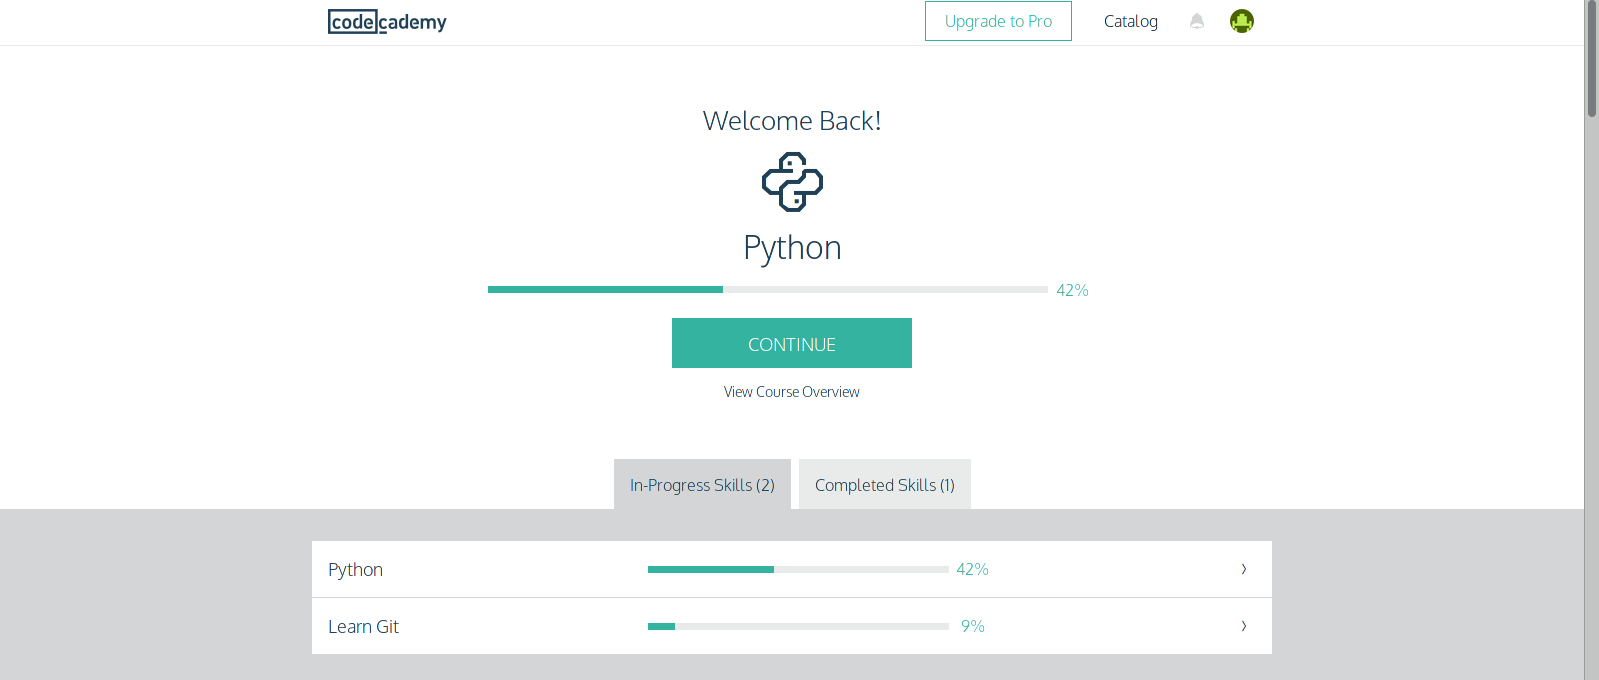
\includegraphics [width=1\linewidth, keepaspectratio =
    1] {./images/sc_web/codeacademy_login_01.png}
    \caption{Zaslonska slika spletne strani
      \emph{\href{https://www.codecademy.com/}{Codeacademy}}
      \cite{web:codeacademy}. Začetna, nadzorna stran po prijavi,
      vidno je na katere tečaje veščin smo prijavljeni in na kolikšnem
    procentu smo ostali. Od tu nadaljujemo na tečaje.}
    \label{fig:scr:web:codeacademy}
\end{figure}

\textbf{Jezik} spletne strani je \textbf{angleščina}, drugi jezikov ni
mogoče izbrati.

Če še podrsamo po spletni strani navzdol, najdemo tečaje, ki učijo
programske jezike in so naslednji: \textbf{HTML + CSS, JavaScript,
  JQuery, PHP, Python, Ruby} in že v prejšnjem odseku so bile na voljo
osnove \textbf{Jave}.

\begin{figure}[h!]
  \centering
    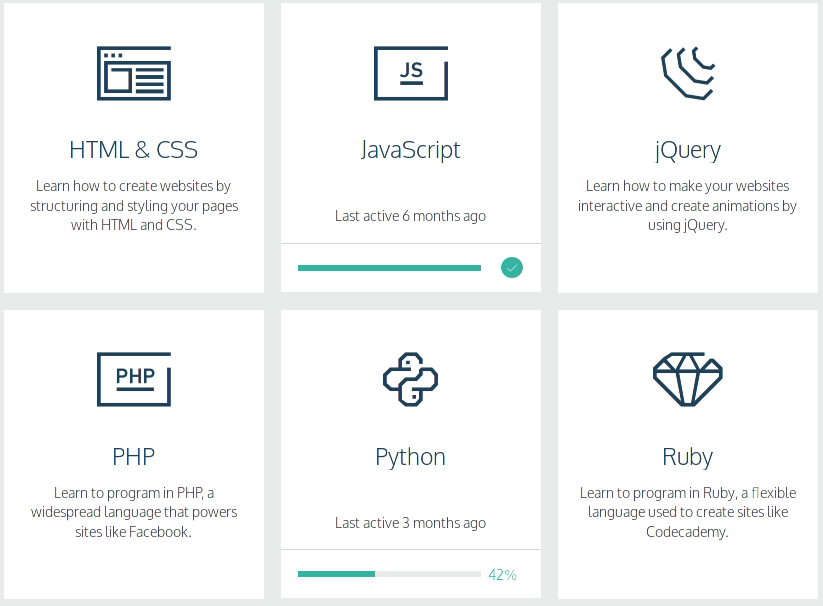
\includegraphics [width=0.65\linewidth, keepaspectratio =
    1] {./images/sc_web/codeacademy_vescine_02.png}
    \caption{Zaslonska slika spletne strani
      \emph{\href{https://www.codecademy.com/}{Codeacademy}}
      \cite{web:codeacademy}. Seznam znanj/veščin programskih jezikov,
      ki jih ponuja spletni portal.}
    \label{fig:scr:web:codeacademy:vescine-prog}
\end{figure}

Nad zbirko osnovnih programskih jezikov najdemo druga
\textbf{ponujenih znanj}, ki jih spletni portal ponuja. V tem delu
najdemo nekatere vsebine kot je na primer, učenje \textbf{SQL},
uporaba \textbf{ukazne vrstice} ali uporabo spletnega orodja za
kontrolo verzije \textbf{GIT}. Nekatere vsebine so sestavljene
projektno, kot je \textbf{Naredi spletno stran} ali \textbf{Naredi
  interaktivno spletno stran}.

% \begin{figure}[h!]
%   \centering
%     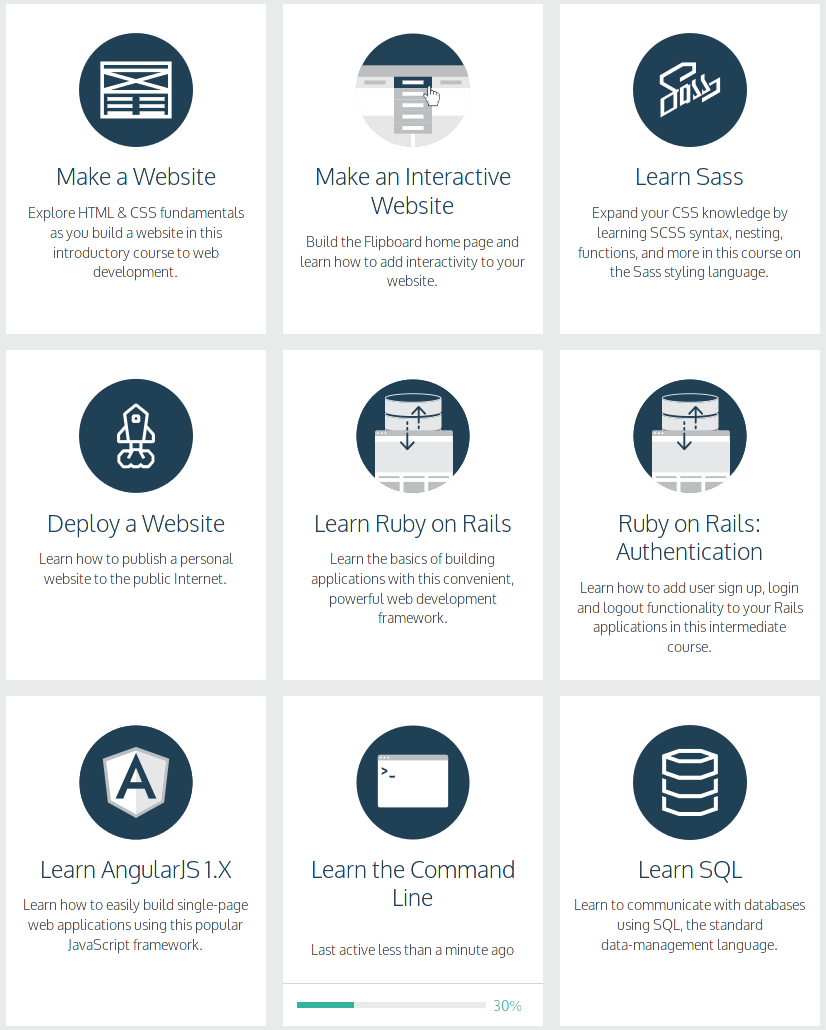
\includegraphics [width=0.65\linewidth, keepaspectratio =
%     1] {./images/sc_web/codeacademy_vescine_01.png}
%     \caption{Zaslonska slika spletne strani
%       \emph{\href{https://www.codecademy.com/}{Codeacademy}}
%       \cite{web:codeacademy}. Seznam znanj/veščin, ki jih ponuja
%       spletni portal.}
%     \label{fig:scr:web:codeacademy:vescine-web}
% \end{figure}

Strnemo lahko, da spletni portal ne ponujajo le znanja in veščine
\textbf{programiranja in programskih jezikov}, temveč tudi druga
znanja. S klikom na želeno vsebino pridemo na stran (slika
\ref{fig:scr:web:codeacademy:tema}), s katere lahko nadaljujemo tam
kjer smo ostali ali pregledujemo posamezne teme, ki smo jih že
opravili ali tiste, ki nas še čakajo.

\begin{figure}[h!]
  \centering
    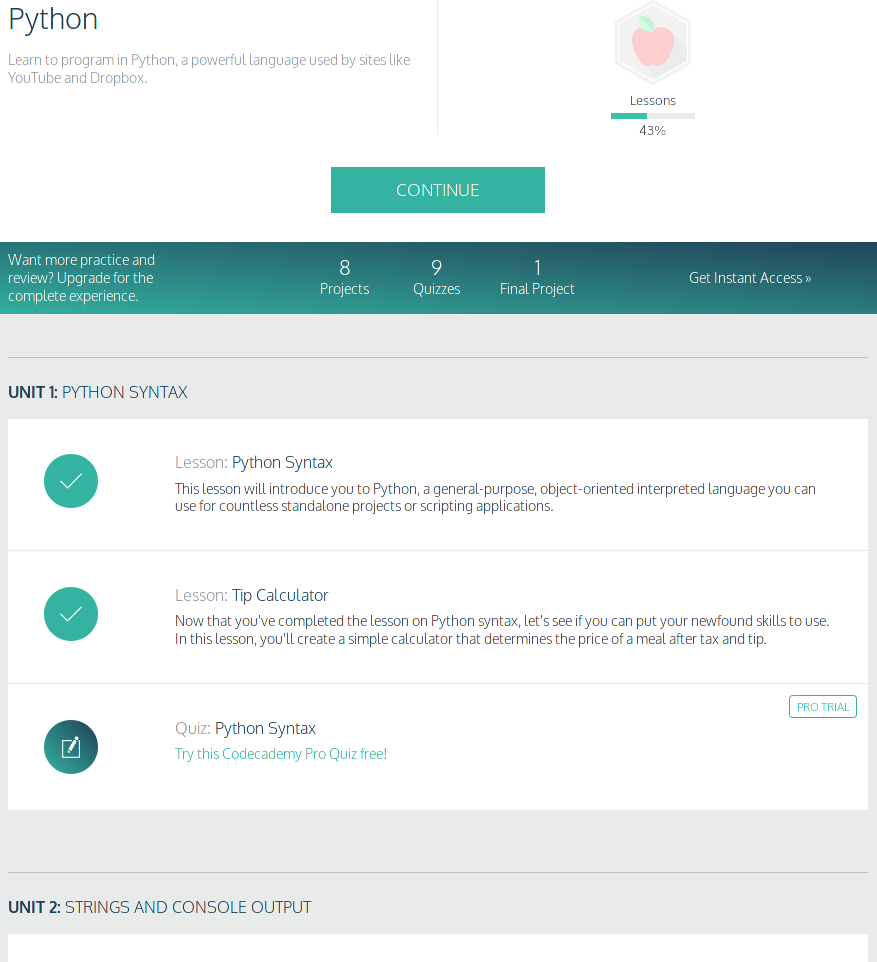
\includegraphics [width=0.65\linewidth, keepaspectratio =
    1] {./images/sc_web/codeacademy_tema_01.png}
    \caption{Zaslonska slika pod strani spletne strani
      \emph{\href{https://www.codecademy.com/}{Codeacademy}}
      \cite{web:codeacademy} na kateri lahko pregledujemo posamezne
      teme in nadaljujemo tam, kjer smo ostali.}
    \label{fig:scr:web:codeacademy:tema}
\end{figure}

Razvidno je, da so teme sistematično razporejene, zato lahko ugotovimo
da je \textbf{načelo sistematičnosti upoštevano}. Z pritiskom na gumb
za nadavaljevanje (\emph{ang. Continue}) odpremo urejevalnik (slika
\ref{fig:scr:web:codeacademy:ide}) na temi in pod enoti na kateri smo
ostali.

\begin{figure}[h!]
  \centering
    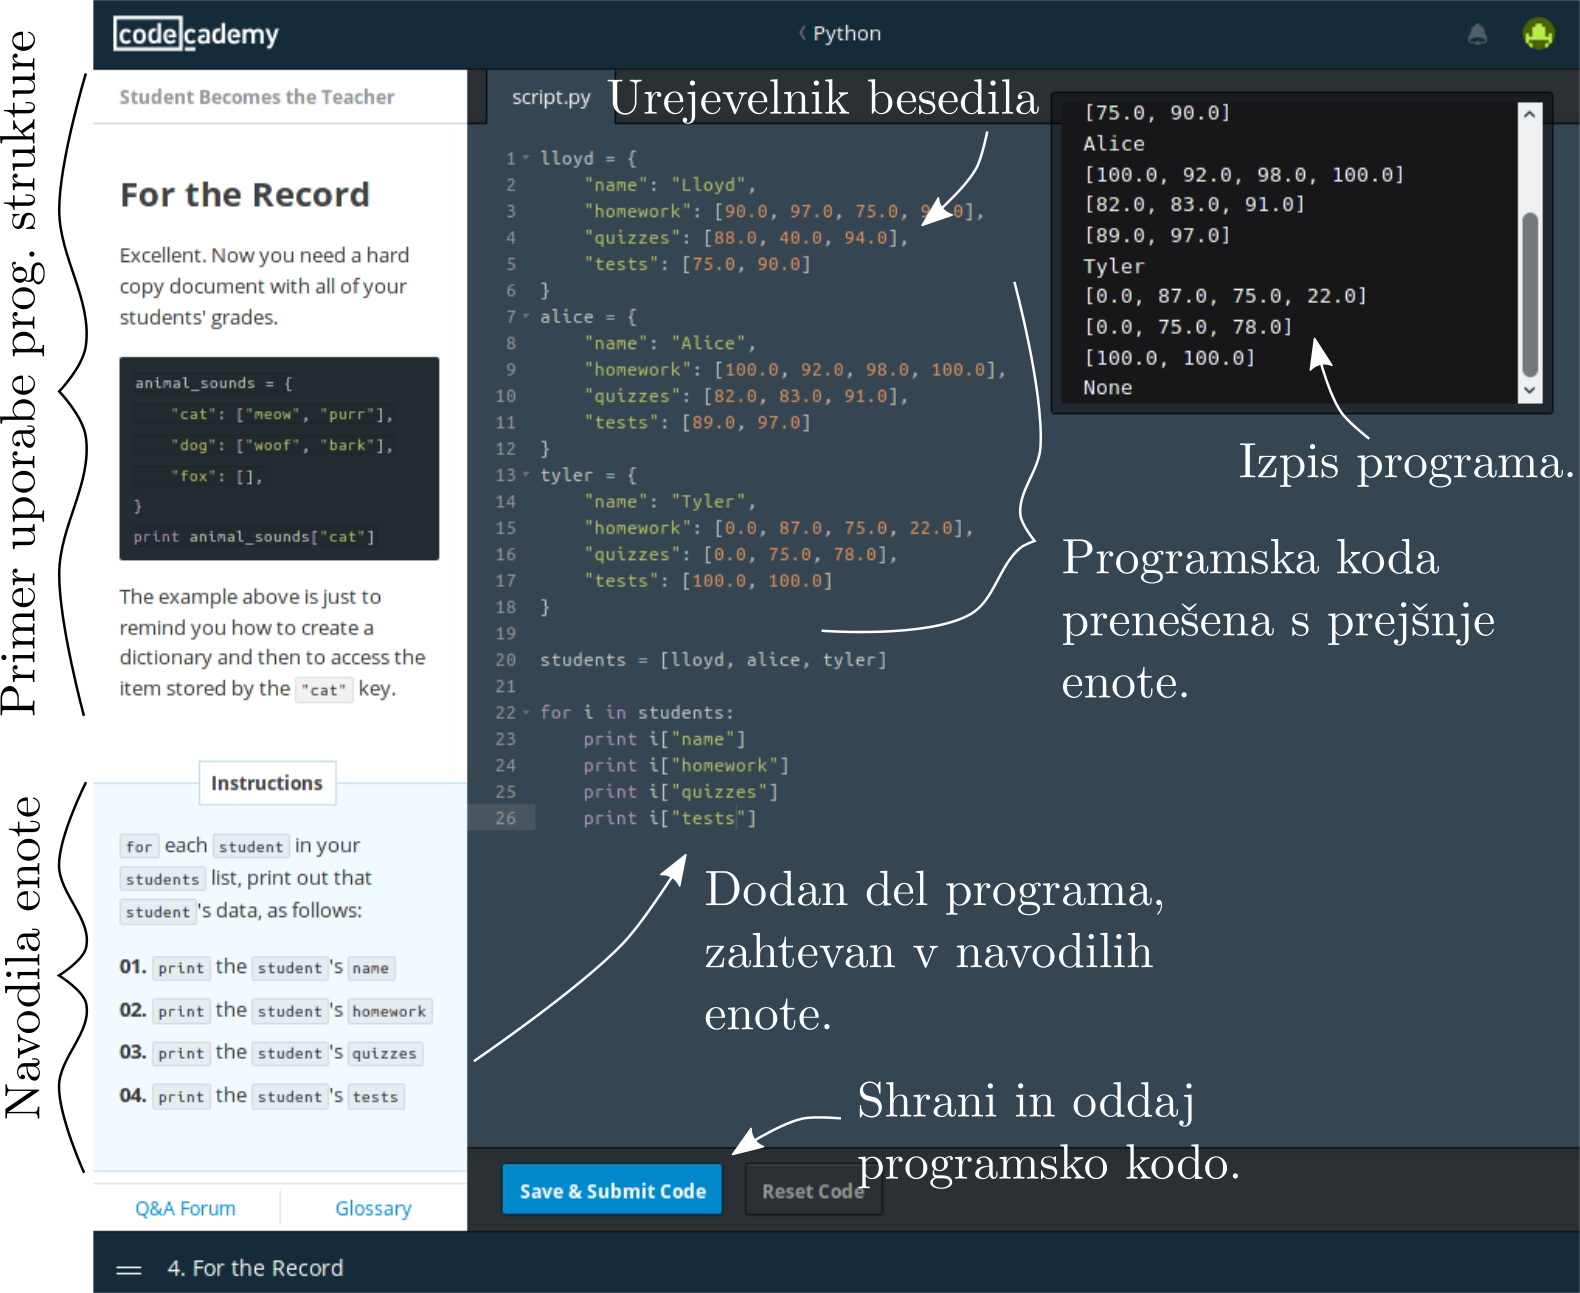
\includegraphics [width=0.65\linewidth, keepaspectratio =
   1] {./images/sc_web/codeacademy_IDE_02.png}
  \caption{Zaslonska slika
      \emph{\href{https://www.codecademy.com/}{Codeacademy}}
      \cite{web:codeacademy} urejevalnika z navodili in python ukazno
      vrstico.} %%NI ukazna vrstica temveč ...
    \label{fig:scr:web:codeacademy:ide}
\end{figure}

Vsaka tema je razdeljena na več enot, ki so sestavljene tako, da
postopoma dograjujejo program. Delo z prejšnje enote se samodejno
prenese naprej. Lahko povemo, da je \textbf{načelo postopnosti}
upoštevano. Pri nekaterih tematskih sklopih sledi najprej ponovitev že
naučenega. Na primer pri Temi \emph{Seznami in funkcije} najprej sledi
pregled osnovnega upravljanja z seznami in pisanjem funkcij.
Uporabniški vmesnik (slika \ref{fig:scr:web:codeacademy:ide}) je
urejen tako, da na desni strani imamo podano snov, ki je sestavljena s
\textbf{primerom določene programske strukture in navodili}, kaj
moramo dograditi v programu. Na levi strani imamo \textbf{urejevalnik
  besedil} v katerega pišemo programsko kodo. Urejevalnik zna barvati
programsko kodo in samodejno predviditi zamike besedila. V zgornjem
desnem kotu je \textbf{okno za izpis} v katerem se izpisujejo
\textbf{izhodni podatki} s programa in napake sintakse \textbf{Pyton
  tolmača}. Spodaj je gumb za \textbf{Shrani in oddaj programsko kode}
(\emph{ang. Save and Submit Code}).

Vsaka ima vedno uvodni del v katerem predstavi neko problematiko, ki
jo potem čez posamezne enote rešujemo. Vsebina je predstavljena
\textbf{problemsko}. Samo delo z \textbf{spletno aplikacijo za
  programiranje} poteka tako, da napišemo program, ki je zahtevan v
navodilih. Ko menimo, da imamo pravilno rešitev pritisnemo na gumb
\textbf{Shrani in oddaj programsko kodo.} Program preverja
\textbf{sintaktično} pravilnost. Napako program vrne nad gumbom za
oddajo programske kode, podrobna napaka \textbf{Pythonov tolmač} se
izpiše v \textbf{oknu za izpis}. Zatem sledi \textbf{semantično}
preverjanje pravilnosti rešitve naloge. V posamezni enoti program
samodejno vrši osnovno preverjanje programa, z točno določeni
rezultatom. Dokler test napisanega programa ne da pravega rezultata me
moremo nadaljevati na naslednjo enoto. Ko se nam zatakne, spletna stran
ponuja \textbf{forum} na katerem najdemo odgovor ali lahko postavimo
vprašanje. Forum je razdeljen na posamezne teme in enote, tako da
lahko hitro najdemo zahtevano vprašanje.



\subsubsection{Povzetek}

\emph{\href{https://www.codecademy.com/}{Codeacademy}}
\cite{web:codeacademy} ima dobro razdelano vsebino, ki je na nekaterih
delih dokaj poglobljena. Sistematičnost, postopnost in problemski
pristop sta prav tako dobro zastavljeni. Portal ponuja številne
projektne vsebine in učenje programskih jezikov. Izbor teh je tak, da
ustreza današnjim spletnim tehnologijam in zahtevam. Znanje se omejuje
predvsem na učenje programiranja ter da se to znanje zna uporabiti v
praktične namene. Spletni portal ima nekatere vsebine in zmožnosti
plačljive, ampak ima zadostno število brezplačnih vsebin, ki omogočajo
normalno delo.


Zanemarjeno je znanje \textbf{Računalniške znanosti}, saj se med
spoznavanjem programskih jezikov in podatkovnih struktur ne uči
različnih algoritmov. Uči se bolj uporabo posameznih funkcij, ki so
vgrajene v programski jezik. Slaba stran spletnega portala je ta, da
je ves v \emph{angleškem jeziku}. Poleg tujega jezika so nekatera
navodila napisana dokaj kompleksno z obratno logiko in zahteva že
dobro poznavanje razumevanja sporočil tolmača in semantičnih napak, ki
se zgodijo v programu.

%Uporaba v šoli.

V primeru učenja programskega jezika \textbf{Python} spletni portal
ponuja zahtevna znanja in je primeren predvsem za srednje in višje
šole. Da bi mentor lahko lahko spletni portal uporabljal pri pouku bi
moral imeti prevode navodil za posamezno za posamezno temo in
enoto. Vsekakor je možno izvesti \emph{praktično vodeno delo}. Mentor
lahko, spletni portal priporoča v uporabo, kot za neobvezno dopolnilno
dejavnost tistim, dijakom, ki želijo razširiti znanje
programiranja. Opozorimo, da jim lahko priporoča le brezplačne
vsebine.


\begin{osebnabox}[label={osebna:codeacademy}]{Codeacademy | \url{www.codeacademy.com}}
    \begin{tabular}{
  p{0.30\linewidth-2\tabcolsep} |
  p{0.70\linewidth-2\tabcolsep}  }
  \textbf{Vrsta vsebine} & Tekstovni vodič, Spletni IDE. \\
      \hline
  \textbf{Jezik spletne strani} &  Angleščina: da, slovenščina: ne. \\
      \hline
  \textbf{Programski jeziki} & Python, ... \\
      \hline
  \textbf{Težavnostna stopnja} & Srednja šola. \\
      \hline
  \textbf{Ponujena znanja ?!} & Znanja programiranja programskih jezikih
      in delo na drugih projektih. \\
      \hline
  \textbf{Upoštevanje načel} & Upošteva načelo sistematičnosti,
      postopnosti, problemski pristop. \\
      \hline
  \textbf{Uporaba dosežkov} & Da. \\
      \hline
  \textbf{Uprabljanje razreda} & Upravljanje razreda je možno. \\
      \hline
  \textbf{Dostop do gradiv} & Delno brezplačen, za napredne projekte je
      potrebno plačevanje naročnine. \\
\end{tabular}
\end{osebnabox}

\section{Ovrednotenje izbranih spletnih portalov in njihove posebnosti}
\label{sec:pregled_spletnih_portalov}


\section{Možni načini uporabe spletnih portalov pri pouku}
\label{sec:načini_uporabe_sp}

%Nekakšen povzetek zgornjih člankov. Vprašanja za naprej.
\subsection{Prednosti pri uporabi SPUP v šoli }
\label{sec:Prednosti_pri_uporavi_SPUP}

% Po pregledu, ki se ukvarjajo z učenjem programiranja lahko
% ugotovimo, da je samo učenje programiranja tanko staro kot prvi
% program, ki je bil kdaj koli napisan.

% NOTE: Razlikovati moramo med kodiranjem in reševanjem problemov
% Začetne misli o učenju programiranja.

% NOTE: Zanima nas naslednja vprašanja:
% NOTE: * Kaj so spletni portali za učenje programiranja?
% NOTE: * Zakaj in kje je smiselno uporabljati spletne portale za
% NOTE:   učenje programiranja.
% NOTE: * Prednosti spletnih portalov in slabosti?
% NOTE: * Kako so spletni portali zgrajeni?
% NOTE: * Katere so različne vrste spletnih portalov (Kategorije) in
% NOTE:   katere bodo nas zanimale?
% NOTE: *

% Kateri tradicionalni spletni portali? Preveri?
% Ali že tu pisati, da v tem primeru gre za učenje na daljavo?!
Tradicionalni spletni portali v izobraževanju, kot so \textbf{moodle},
nikoli niso popolnoma izkoristili zmožnosti uporabe, ki jih ponujajo
nove internetne in komunikacijske tehnologije. Večinoma so se
uporabljale le kot podaljšana roka obstoječim metodam
poučevanja. Uporabljale so se za objavo gradiv in spletno prijavo za
oddajo nalog. Takšni sistemi ne zagotavljajo izboljšav kvalitete
poučevanja programiranja \cite{ITaLCP_DistanceEdu}.

Strnimo nekatere značilnosti težav novincev.

\begin{itemize}
\tightlist
\item Težave pri namestitvi in nastavitvah programske opreme,
  prevajalnika in razvojnega okolja (OUHK, QUTA ).
\item Dostop do mentorjev zaradi časovne dostopnosti in Komunikacija v
  primeru izobraževanja na daljavo (OUHK, QUTA).
\item Uporaba urejevalnika besedil (QUTA).
\item Razumevanje programskih vprašanj in uprabe sintakse jezika pri
  pisanj programske kode (QUTA).
\item Uporoaba tehnik razhroščevanje (QUTA).
\item Razumevanje napak prevajalnika (QUTA).
\item Razumevanje osnovnih programskih koceptov, slabo vpliva na
  reševanje koceptov (US).
\end{itemize}

S težavami novince se lahko poistovetijo tudi učenci in dijaki, ki začnejo z
učenjem programiranja. Rešitve, ki jih je uporaba SPUP prinesla na
univerze lahko prenesemo na uporabo v osnovno in srednjo
šolo. Naštejemo lahko nekatere prednosti, ki bi jih taka uporaba lahko
imela.

\subsubsection{Namestitev programske opreme}
\label{sec:Namestitev_programske_opreme}

Med prvimi prednostmi je sigurno namestitev potrebne programske
opreme. Učitelju praktično ni potrebno nameščati nobenega urejevalnika
besedil, IDE, niti prevajalnika ali tolmača. Prav tako ni potrebe po
nastavljanju sistemskih poti, ki jih mnogi prevajalniki zahtevajo.

Uporaba SPUP je neodvisna od uporabe operacijskega sistema. Vsaka
naprava, na kateri lahko poganjamo spletni brskalnik omogoča uporabo
SPUP.

Velika prednost, da ni potrebe po instalaciji programske opreme je
tudi za učence, saj jim doma ni potrebno nalagati nobenega
programa. Na tem mestu bi poudarili, da učitelj mora biti previden pri
dajanju domače naloge z uporabo računalnika. Zares se mora prepričati,
da to zmožnost imajo vsi učenci. Najbolje je da vso dodatno delo, ki
ga učitelj predvidi lahko učenci opravijo v šolski računalniški
učilnici.

\subsubsection{Seznanjanje s programsko opremo}
\label{sec:Seznanjanje_s_prog_opremo}

Za učence ni potrebe, da bi spoznavali urejevalnik besedil ali
IDE. Spoznavanja programskega jezika in reševanje problemov se lahko
lotijo nemudoma.


\subsubsection{Pisanje programa od začetka do konca ni potrebno}
\label{sec:pisanj_celega_progama}

Večina spletnih portalov, ki ponujajo vsebine, imajo programske naloge
pripravljene tako, da uporabnik mora vnesti le del programske kode. Za
novinca, to pomeni, da se koncentrira le na nalogo in del sintakse, ki
jo v danem trenutku potrebuje, da reši zadano nalogo. To prednost smo
že spoznali na SPUP avstralske univerze, kjer so uporabili, tip
naloge, zapolni prazna mesta \cite{thesisAWebP}.

%To mogoče ne spada sem saj je bolj specifićen feature.
\subsubsection{Nagrajevanje z dosežki}
\label{sec:nagrajevanje_s_dosežkov}






%%% Local Variables:
%%% mode: latex
%%% TeX-master: "diploma"o ostali ali pregledujemo posamezne enote, ki smo jih že
opravili ali tiste, ki nas še čakajo.

\begin{figure}[h!]
  \centering
    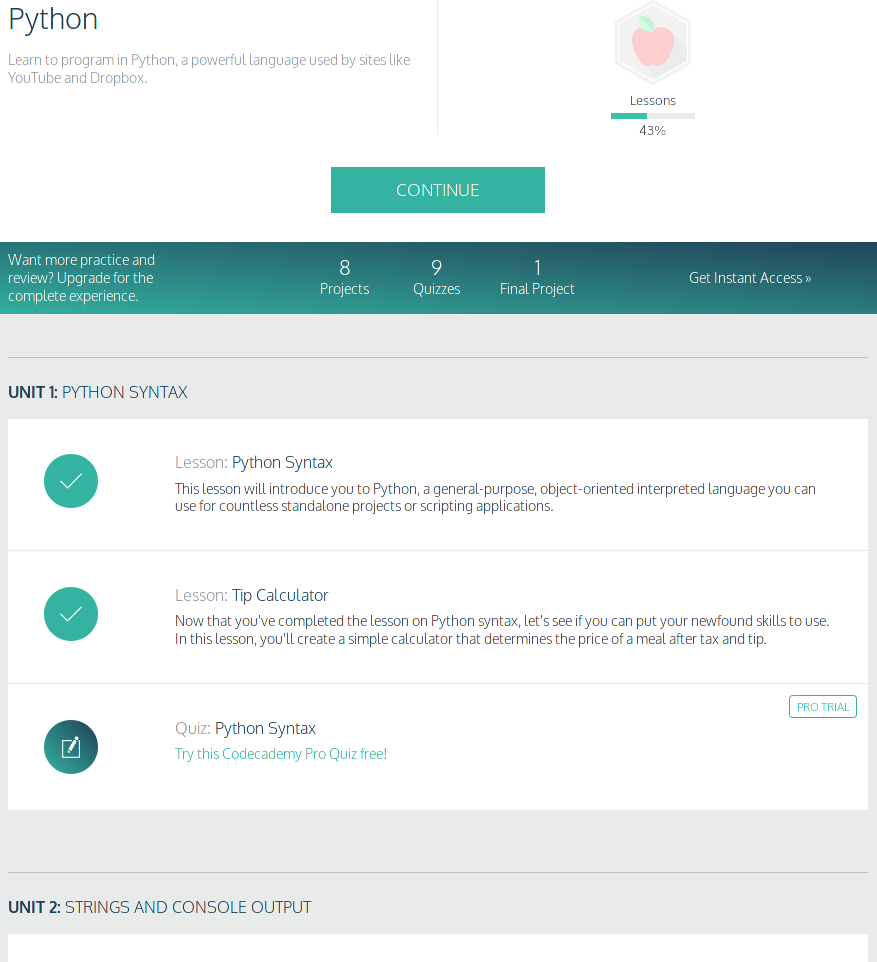
\includegraphics [width=0.65\linewidth, keepaspectratio =
    1] {./images/sc_web/codeacademy_tema_01.png}
    \caption{Zaslonska slika pod strani spletne strani
      \emph{\href{https://www.codecademy.com/}{Codeacademy}}
      \cite{web:codeacademy} na kateri lahko pregledujemo posamezne
      enote in nadaljujemo tam, kjer smo ostali.}
    \label{fig:scr:web:codeacademy:tema}
\end{figure}



\subsubsection{Povzetek}

\begin{osebnabox}[label={osebna:codeacademy}]{Codeacademy | \url{www.codeacademy.com}}
    \begin{tabular}{
  p{0.30\linewidth-2\tabcolsep} |
  p{0.70\linewidth-2\tabcolsep}  }
  \textbf{Vrsta vsebine} & Tekstovni vodič, Spletni IDE. \\
      \hline
  \textbf{Jezik spletne strani} &  Angleščina: da, slovenščina: ne. \\
      \hline
  \textbf{Programski jeziki} & Python, ... \\
      \hline
  \textbf{Težavnostna stopnja} & Srednja šola. \\
      \hline
  \textbf{Ponujena znanja ?!} & Znanja programiranja programskih jezikih
      in delo na drugih projektih. \\
      \hline
  \textbf{Upoštevanje načel} & Upošteva načelo sistematičnosti,
      postopnosti, problemski pristop. \\
      \hline
  \textbf{Uporaba dosežkov} & Da. \\
      \hline
  \textbf{Uprabljanje razreda} & Upravljanje razreda je možno. \\
      \hline
  \textbf{Dostop do gradiv} & Delno brezplačen, za napredne projekte je
      potrebno plačevanje naročnine. \\
\end{tabular}
\end{osebnabox}

\section{Ovrednotenje izbranih spletnih portalov in njihove posebnosti}
\label{sec:pregled_spletnih_portalov}


\section{Možni načini uporabe spletnih portalov pri pouku}
\label{sec:načini_uporabe_sp}

%Nekakšen povzetek zgornjih člankov. Vprašanja za naprej.
\subsection{Prednosti pri uporabi SPUP v šoli }
\label{sec:Prednosti_pri_uporavi_SPUP}

% Po pregledu, ki se ukvarjajo z učenjem programiranja lahko
% ugotovimo, da je samo učenje programiranja tanko staro kot prvi
% program, ki je bil kdaj koli napisan.

% NOTE: Razlikovati moramo med kodiranjem in reševanjem problemov
% Začetne misli o učenju programiranja.

% NOTE: Zanima nas naslednja vprašanja:
% NOTE: * Kaj so spletni portali za učenje programiranja?
% NOTE: * Zakaj in kje je smiselno uporabljati spletne portale za
% NOTE:   učenje programiranja.
% NOTE: * Prednosti spletnih portalov in slabosti?
% NOTE: * Kako so spletni portali zgrajeni?
% NOTE: * Katere so različne vrste spletnih portalov (Kategorije) in
% NOTE:   katere bodo nas zanimale?
% NOTE: *

% Kateri tradicionalni spletni portali? Preveri?
% Ali že tu pisati, da v tem primeru gre za učenje na daljavo?!
Tradicionalni spletni portali v izobraževanju, kot so \textbf{moodle},
nikoli niso popolnoma izkoristili zmožnosti uporabe, ki jih ponujajo
nove internetne in komunikacijske tehnologije. Večinoma so se
uporabljale le kot podaljšana roka obstoječim metodam
poučevanja. Uporabljale so se za objavo gradiv in spletno prijavo za
oddajo nalog. Takšni sistemi ne zagotavljajo izboljšav kvalitete
poučevanja programiranja \cite{ITaLCP_DistanceEdu}.

Strnimo nekatere značilnosti težav novincev.

\begin{itemize}
\tightlist
\item Težave pri namestitvi in nastavitvah programske opreme,
  prevajalnika in razvojnega okolja (OUHK, QUTA ).
\item Dostop do mentorjev zaradi časovne dostopnosti in Komunikacija v
  primeru izobraževanja na daljavo (OUHK, QUTA).
\item Uporaba urejevalnika besedil (QUTA).
\item Razumevanje programskih vprašanj in uprabe sintakse jezika pri
  pisanj programske kode (QUTA).
\item Uporoaba tehnik razhroščevanje (QUTA).
\item Razumevanje napak prevajalnika (QUTA).
\item Razumevanje osnovnih programskih koceptov, slabo vpliva na
  reševanje koceptov (US).
\end{itemize}

S težavami novince se lahko poistovetijo tudi učenci in dijaki, ki začnejo z
učenjem programiranja. Rešitve, ki jih je uporaba SPUP prinesla na
univerze lahko prenesemo na uporabo v osnovno in srednjo
šolo. Naštejemo lahko nekatere prednosti, ki bi jih taka uporaba lahko
imela.

\subsubsection{Namestitev programske opreme}
\label{sec:Namestitev_programske_opreme}

Med prvimi prednostmi je sigurno namestitev potrebne programske
opreme. Učitelju praktično ni potrebno nameščati nobenega urejevalnika
besedil, IDE, niti prevajalnika ali tolmača. Prav tako ni potrebe po
nastavljanju sistemskih poti, ki jih mnogi prevajalniki zahtevajo.

Uporaba SPUP je neodvisna od uporabe operacijskega sistema. Vsaka
naprava, na kateri lahko poganjamo spletni brskalnik omogoča uporabo
SPUP.

Velika prednost, da ni potrebe po instalaciji programske opreme je
tudi za učence, saj jim doma ni potrebno nalagati nobenega
programa. Na tem mestu bi poudarili, da učitelj mora biti previden pri
dajanju domače naloge z uporabo računalnika. Zares se mora prepričati,
da to zmožnost imajo vsi učenci. Najbolje je da vso dodatno delo, ki
ga učitelj predvidi lahko učenci opravijo v šolski računalniški
učilnici.

\subsubsection{Seznanjanje s programsko opremo}
\label{sec:Seznanjanje_s_prog_opremo}

Za učence ni potrebe, da bi spoznavali urejevalnik besedil ali
IDE. Spoznavanja programskega jezika in reševanje problemov se lahko
lotijo nemudoma.


\subsubsection{Pisanje programa od začetka do konca ni potrebno}
\label{sec:pisanj_celega_progama}

Večina spletnih portalov, ki ponujajo vsebine, imajo programske naloge
pripravljene tako, da uporabnik mora vnesti le del programske kode. Za
novinca, to pomeni, da se koncentrira le na nalogo in del sintakse, ki
jo v danem trenutku potrebuje, da reši zadano nalogo. To prednost smo
že spoznali na SPUP avstralske univerze, kjer so uporabili, tip
naloge, zapolni prazna mesta \cite{thesisAWebP}.

%To mogoče ne spada sem saj je bolj specifićen feature.
\subsubsection{Nagrajevanje z dosežki}
\label{sec:nagrajevanje_s_dosežkov}

% \newpage
% %%Recept za vstavljanje poljubnega naslova za Viri in literatura
\cleardoublepage
\renewcommand*{\refname}{Literatura in viri}
% %\renewcommand*{\refname}{\vspace*{-12mm}}
% %\section*{Viri in Literatura}
%\phantomsection
%\addcontentsline{toc}{section}{Literatura in viri}
% %\addcontentsline{toc}{section}{Literatura}
\begin{thebibliography}{9}

% NOTE: Citiranje sem povzel po ieee z dokumenta ieeecitationref.pdf.
% NOTE: Spodaj dodajam
%
%nekaj uporabljenih primerov člankov, ki jih
% NOTE: bom potrebovalmm

% TODO: Prosi za pomoč pri oblikovanju in uporabi literature.

\bibitem{model_uporabe_rac_izo-web}
  Martina Fefer,
  \emph{Uporaba informacijske-komunikacijske  tehnologije v osnovnih
    šolah s prilagojenim programom},
  Univerza v Mariboru - Fakulteta za naravoslovje in matematiko, Maribor,
  1999. Pridobljeno 4.4. 2016, iz \url{http://student.pfmb.uni-mb.si/~dgunze/diplomske/d2/s6.html}.

\bibitem{LTProg01}
  Anthony Robins, Janet Rountree, and Nathan Rountree,
  ''Learning and Teaching Programming: A Review and
  Discussion'' v \emph{Comuper Science education}, vol 13, No. 2,
  2003, pp. 137 - 172.
  % Univerza: Computer Science, University of Otago, Dunedin, New Zealand.

\bibitem{ITaLCP_DistanceEdu}
  S.C. Ng, S.O Choy, R. Kwan, S.F. Chan,
  ''A Web-Based Environment to Improve Teaching and Learning of
  Computer Programming in Distance Education'', \emph{ICWL'05
    Proceedings of the 4th international conference on Advances in
    Web-Based Learning}, 2005

\bibitem{mentalModels}
  - L. Ma, J. D. Ferguson, M. Roper, I.Ross, M. Wood,
  ''A web-based learning model for improving programming students' mental
  models'', v \emph{Proceedings of the 9th annual conference of the subject
  centre for information and computer sciences}, HE Academy, 2008
  pp. 88-94.

\bibitem{guideTCS}
  O. Hazzan, T. Lapidot, N. Ragonis,
  \emph{Guide to Teaching Computer Science}, Springer, 2011.

\bibitem{thesisAWebP}
  Nghi Truong,
  \emph{A web-based programming environment for novice programmers},
  Queensland University of Technology, Australia, 2007.



% \bibitem{bilten01}
%   \emph{Tematska številka Biltena E-šolstvo}, \\
%   Bilten E-šolstva, Številka: 2010/1\\
%  elektronski vir: \url{http://projekt.sio.si/wp-content/uploads/sites/8/2015/01/E-solstvo_BILTEN_2010-1_screen.pd}\\
% (E-središče v okviru projekta E-šolstvo, 2010)

% \bibitem{test}
%  CPI, \emph{O CPI}, \\
%   \url{http://www.cpi.si/o-cpi.aspx},\\
%   Obiskano: \emph{\datum}

%  \bibitem{esolska_torba}
%   SIO, \emph{E-šolska torba}, \\
%    \url{http://projekt.sio.si/e-solska-torba/},\\
%    Obiskano: \emph{\datum}

%  \bibitem{sio_arhiv}
%   SIO, \emph{Repozitorij gradiv}, \\
%    \url{http://portal.sio.si/no_cache/sio/gradiva/repozitorij_gradiv_trubar/},\\
%    Obiskano: \emph{\datum}

%  \bibitem{stran_execute}
%   \emph{Spletna stran execute}, \\
%    \url{http://execute.fnm.uni-mb.si},\\
%    Obiskano: \emph{\datum}


% \bibitem{iUčbeniki}
%   Andreja Čuk ... [et al.], \\
%   \emph{SLOVENSKI i-učbeniki} [elektronski vir], \\
%   način dostopa: \url{http://www.zrss.si/pdf/slovenski-i-ucbeniki.pdf}\\
%   (Zavod republike slovenije za šolstvo, 2014)


% \bibitem{dipl_simulacije1}
%   Vera Kožuh \\
%   \emph{Diplomska seminarska naloga - Simulacije z računalnikom pri
%     pouku fizike v osnovni šoli}, \\
%  elektronski vir: \url{http://splet-stari.fnm.uni-mb.si/pefmb_old/didgradiva/diplome/kozuh/}\\
% (Pedagoška fakulteta - Oddelek za fiziko, Maribor 1999)


% \bibitem{informatika_2010}
%   Avtor, \\
%   \emph{Naslov} \\
% (Založba, Mesto 2006)



\end{thebibliography}


  %%% Local Variables:
  %%% mode: latex
  %%% TeX-master: "diploma"
  %%% End:





%%% End document
\end{document}


%%% Local Variables:
%%% mode: latex
%%% TeX-master: t
%%% End:
